\documentclass[11pt]{article}
\usepackage[T1]{fontenc}
\usepackage[utf8]{inputenc}
\usepackage{lmodern}
\usepackage[a4paper,margin=2.3cm]{geometry}
\usepackage{amsmath,amssymb}
\usepackage{graphicx}
\usepackage{booktabs}
\usepackage{multirow}
\usepackage{xcolor}
\usepackage{caption}
\usepackage{subcaption}
\usepackage{siunitx}
\usepackage[numbers,sort&compress]{natbib}
\usepackage[colorlinks=true,linkcolor=blue!50!black,citecolor=blue!50!black,urlcolor=blue!50!black]{hyperref}
\captionsetup{font=small,labelfont=bf}
\graphicspath{{figures/}}
\sisetup{detect-all}

% Generado por scripts/11_figures_tables.py: no editar a mano.
\newcommand{\AllAuc}{0.57}
\newcommand{\AllAucHi}{0.72}
\newcommand{\AllAucLo}{0.42}
\newcommand{\AllP}{0.278}
\newcommand{\BestModelKey}{LrLAll}
\newcommand{\BestModelName}{LR-L1, all features}
\newcommand{\BySexFemaleAuc}{0.56}
\newcommand{\BySexFemaleN}{16}
\newcommand{\BySexMaleAuc}{0.51}
\newcommand{\BySexMaleN}{29}
\newcommand{\CmpDlEegnetVsDemoDiff}{-0.33}
\newcommand{\CmpDlEegnetVsDemoP}{0.022}
\newcommand{\CmpDlEegnetVsPrimaryDiff}{-0.09}
\newcommand{\CmpDlEegnetVsPrimaryP}{0.512}
\newcommand{\CmpDlShallowfbcspnetVsDemoDiff}{-0.36}
\newcommand{\CmpDlShallowfbcspnetVsDemoP}{0.025}
\newcommand{\CmpDlShallowfbcspnetVsPrimaryDiff}{-0.12}
\newcommand{\CmpDlShallowfbcspnetVsPrimaryP}{0.434}
\newcommand{\CmpDlTcnVsDemoDiff}{-0.31}
\newcommand{\CmpDlTcnVsDemoP}{0.078}
\newcommand{\CmpDlTcnVsPrimaryDiff}{-0.07}
\newcommand{\CmpDlTcnVsPrimaryP}{0.656}
\newcommand{\CmpErpcovTsLrVsDemoDiff}{-0.17}
\newcommand{\CmpErpcovTsLrVsDemoP}{0.164}
\newcommand{\CmpErpcovTsLrVsPrimaryDiff}{+0.08}
\newcommand{\CmpErpcovTsLrVsPrimaryP}{0.455}
\newcommand{\CmpLightgbmAllVsDemoDiff}{-0.24}
\newcommand{\CmpLightgbmAllVsDemoP}{0.020}
\newcommand{\CmpLightgbmAllVsPrimaryDiff}{+0.01}
\newcommand{\CmpLightgbmAllVsPrimaryP}{0.944}
\newcommand{\CmpLrLAllVsDemoDiff}{-0.09}
\newcommand{\CmpLrLAllVsDemoP}{0.470}
\newcommand{\CmpLrLAllVsPrimaryDiff}{+0.16}
\newcommand{\CmpLrLAllVsPrimaryP}{0.106}
\newcommand{\CmpLrLComplexityVsDemoDiff}{-0.19}
\newcommand{\CmpLrLComplexityVsDemoP}{0.107}
\newcommand{\CmpLrLComplexityVsPrimaryDiff}{+0.06}
\newcommand{\CmpLrLComplexityVsPrimaryP}{0.517}
\newcommand{\CmpLrLConnectivityVsDemoDiff}{-0.34}
\newcommand{\CmpLrLConnectivityVsDemoP}{0.008}
\newcommand{\CmpLrLConnectivityVsPrimaryDiff}{-0.10}
\newcommand{\CmpLrLConnectivityVsPrimaryP}{0.325}
\newcommand{\CmpLrLErpVsDemoDiff}{-0.40}
\newcommand{\CmpLrLErpVsDemoP}{0.000}
\newcommand{\CmpLrLErpVsPrimaryDiff}{-0.15}
\newcommand{\CmpLrLErpVsPrimaryP}{0.121}
\newcommand{\CmpLrLSpectralVsDemoDiff}{-0.26}
\newcommand{\CmpLrLSpectralVsDemoP}{0.011}
\newcommand{\CmpLrLSpectralVsPrimaryDiff}{-0.01}
\newcommand{\CmpLrLSpectralVsPrimaryP}{0.903}
\newcommand{\CmpMdmVsDemoDiff}{-0.44}
\newcommand{\CmpMdmVsDemoP}{0.000}
\newcommand{\CmpMdmVsPrimaryDiff}{-0.19}
\newcommand{\CmpMdmVsPrimaryP}{0.094}
\newcommand{\CmpNestedmodelselectionAllVsDemoDiff}{-0.17}
\newcommand{\CmpNestedmodelselectionAllVsDemoP}{0.176}
\newcommand{\CmpNestedmodelselectionAllVsPrimaryDiff}{+0.08}
\newcommand{\CmpNestedmodelselectionAllVsPrimaryP}{0.392}
\newcommand{\CmpPrimaryLrLAllVsDemoDiff}{-0.25}
\newcommand{\CmpPrimaryLrLAllVsDemoP}{0.019}
\newcommand{\CmpRandomforestAllVsDemoDiff}{-0.22}
\newcommand{\CmpRandomforestAllVsDemoP}{0.029}
\newcommand{\CmpRandomforestAllVsPrimaryDiff}{+0.02}
\newcommand{\CmpRandomforestAllVsPrimaryP}{0.672}
\newcommand{\CmpSvmLinearAllVsDemoDiff}{-0.38}
\newcommand{\CmpSvmLinearAllVsDemoP}{0.004}
\newcommand{\CmpSvmLinearAllVsPrimaryDiff}{-0.13}
\newcommand{\CmpSvmLinearAllVsPrimaryP}{0.422}
\newcommand{\CmpSvmRbfAllVsDemoDiff}{-0.38}
\newcommand{\CmpSvmRbfAllVsDemoP}{0.008}
\newcommand{\CmpSvmRbfAllVsPrimaryDiff}{-0.13}
\newcommand{\CmpSvmRbfAllVsPrimaryP}{0.429}
\newcommand{\CmpTsLrVsDemoDiff}{-0.30}
\newcommand{\CmpTsLrVsDemoP}{0.027}
\newcommand{\CmpTsLrVsPrimaryDiff}{-0.05}
\newcommand{\CmpTsLrVsPrimaryP}{0.670}
\newcommand{\ConfAgeAuc}{0.50}
\newcommand{\ConfAgeAucHi}{0.67}
\newcommand{\ConfAgeAucLo}{0.33}
\newcommand{\ConfAgeP}{0.617}
\newcommand{\ConfRecordingAuc}{0.55}
\newcommand{\ConfRecordingAucHi}{0.72}
\newcommand{\ConfRecordingAucLo}{0.37}
\newcommand{\ConfRecordingP}{0.392}
\newcommand{\ConfSexAuc}{0.63}
\newcommand{\ConfSexAucHi}{0.79}
\newcommand{\ConfSexAucLo}{0.45}
\newcommand{\ConfSexP}{0.018}
\newcommand{\DemoAgeP}{0.823}
\newcommand{\DemoEducationP}{0.005}
\newcommand{\DemoGadP}{0.000}
\newcommand{\DemoGenderP}{0.394}
\newcommand{\DemoPhqP}{0.000}
\newcommand{\DemoPsqiP}{0.000}
\newcommand{\DemographicsLrAuc}{0.78}
\newcommand{\DemographicsLrAucHi}{0.91}
\newcommand{\DemographicsLrAucLo}{0.63}
\newcommand{\DemographicsLrAucSd}{0.04}
\newcommand{\DemographicsLrBalancedAccuracy}{0.76}
\newcommand{\DemographicsLrBalancedAccuracyHi}{0.88}
\newcommand{\DemographicsLrBalancedAccuracyLo}{0.63}
\newcommand{\DemographicsLrBrier}{0.205}
\newcommand{\DemographicsLrBrierHi}{0.259}
\newcommand{\DemographicsLrBrierLo}{0.157}
\newcommand{\DemographicsLrF}{0.71}
\newcommand{\DemographicsLrFHi}{0.86}
\newcommand{\DemographicsLrFLo}{0.55}
\newcommand{\DemographicsLrNperm}{1000}
\newcommand{\DemographicsLrNullQ}{0.66}
\newcommand{\DemographicsLrPperm}{0.002}
\newcommand{\DemographicsLrSensitivity}{0.72}
\newcommand{\DemographicsLrSensitivityHi}{0.91}
\newcommand{\DemographicsLrSensitivityLo}{0.51}
\newcommand{\DemographicsLrSpecificity}{0.80}
\newcommand{\DemographicsLrSpecificityHi}{0.95}
\newcommand{\DemographicsLrSpecificityLo}{0.65}
\newcommand{\DlEegnetAuc}{0.47}
\newcommand{\DlEegnetAucHi}{0.65}
\newcommand{\DlEegnetAucLo}{0.30}
\newcommand{\DlEegnetAucSd}{0.09}
\newcommand{\DlEegnetBalancedAccuracy}{0.46}
\newcommand{\DlEegnetBalancedAccuracyHi}{0.58}
\newcommand{\DlEegnetBalancedAccuracyLo}{0.35}
\newcommand{\DlEegnetBrier}{0.324}
\newcommand{\DlEegnetBrierHi}{0.398}
\newcommand{\DlEegnetBrierLo}{0.256}
\newcommand{\DlEegnetF}{0.20}
\newcommand{\DlEegnetFHi}{0.39}
\newcommand{\DlEegnetFLo}{0.05}
\newcommand{\DlEegnetNperm}{0}
\newcommand{\DlEegnetPperm}{--}
\newcommand{\DlEegnetSensitivity}{0.17}
\newcommand{\DlEegnetSensitivityHi}{0.33}
\newcommand{\DlEegnetSensitivityLo}{0.04}
\newcommand{\DlEegnetSpecificity}{0.75}
\newcommand{\DlEegnetSpecificityHi}{0.90}
\newcommand{\DlEegnetSpecificityLo}{0.58}
\newcommand{\DlShallowfbcspnetAuc}{0.44}
\newcommand{\DlShallowfbcspnetAucHi}{0.61}
\newcommand{\DlShallowfbcspnetAucLo}{0.27}
\newcommand{\DlShallowfbcspnetAucSd}{0.08}
\newcommand{\DlShallowfbcspnetBalancedAccuracy}{0.48}
\newcommand{\DlShallowfbcspnetBalancedAccuracyHi}{0.62}
\newcommand{\DlShallowfbcspnetBalancedAccuracyLo}{0.35}
\newcommand{\DlShallowfbcspnetBrier}{0.350}
\newcommand{\DlShallowfbcspnetBrierHi}{0.441}
\newcommand{\DlShallowfbcspnetBrierLo}{0.267}
\newcommand{\DlShallowfbcspnetF}{0.34}
\newcommand{\DlShallowfbcspnetFHi}{0.53}
\newcommand{\DlShallowfbcspnetFLo}{0.14}
\newcommand{\DlShallowfbcspnetNperm}{0}
\newcommand{\DlShallowfbcspnetPperm}{--}
\newcommand{\DlShallowfbcspnetSensitivity}{0.31}
\newcommand{\DlShallowfbcspnetSensitivityHi}{0.52}
\newcommand{\DlShallowfbcspnetSensitivityLo}{0.11}
\newcommand{\DlShallowfbcspnetSpecificity}{0.65}
\newcommand{\DlShallowfbcspnetSpecificityHi}{0.83}
\newcommand{\DlShallowfbcspnetSpecificityLo}{0.47}
\newcommand{\DlTcnAuc}{0.48}
\newcommand{\DlTcnAucHi}{0.65}
\newcommand{\DlTcnAucLo}{0.30}
\newcommand{\DlTcnAucSd}{0.05}
\newcommand{\DlTcnBalancedAccuracy}{0.48}
\newcommand{\DlTcnBalancedAccuracyHi}{0.63}
\newcommand{\DlTcnBalancedAccuracyLo}{0.34}
\newcommand{\DlTcnBrier}{0.287}
\newcommand{\DlTcnBrierHi}{0.343}
\newcommand{\DlTcnBrierLo}{0.233}
\newcommand{\DlTcnF}{0.39}
\newcommand{\DlTcnFHi}{0.56}
\newcommand{\DlTcnFLo}{0.19}
\newcommand{\DlTcnNperm}{0}
\newcommand{\DlTcnPperm}{--}
\newcommand{\DlTcnSensitivity}{0.41}
\newcommand{\DlTcnSensitivityHi}{0.63}
\newcommand{\DlTcnSensitivityLo}{0.19}
\newcommand{\DlTcnSpecificity}{0.56}
\newcommand{\DlTcnSpecificityHi}{0.74}
\newcommand{\DlTcnSpecificityLo}{0.37}
\newcommand{\ErpClusterMinP}{0.31}
\newcommand{\ErpNClusters}{52}
\newcommand{\ErpcovTsLrAuc}{0.61}
\newcommand{\ErpcovTsLrAucHi}{0.78}
\newcommand{\ErpcovTsLrAucLo}{0.43}
\newcommand{\ErpcovTsLrAucSd}{0.03}
\newcommand{\ErpcovTsLrBalancedAccuracy}{0.56}
\newcommand{\ErpcovTsLrBalancedAccuracyHi}{0.70}
\newcommand{\ErpcovTsLrBalancedAccuracyLo}{0.42}
\newcommand{\ErpcovTsLrBrier}{0.246}
\newcommand{\ErpcovTsLrBrierHi}{0.307}
\newcommand{\ErpcovTsLrBrierLo}{0.188}
\newcommand{\ErpcovTsLrF}{0.46}
\newcommand{\ErpcovTsLrFHi}{0.64}
\newcommand{\ErpcovTsLrFLo}{0.25}
\newcommand{\ErpcovTsLrNperm}{200}
\newcommand{\ErpcovTsLrNullQ}{0.67}
\newcommand{\ErpcovTsLrPholm}{1.000}
\newcommand{\ErpcovTsLrPperm}{0.159}
\newcommand{\ErpcovTsLrSensitivity}{0.44}
\newcommand{\ErpcovTsLrSensitivityHi}{0.67}
\newcommand{\ErpcovTsLrSensitivityLo}{0.22}
\newcommand{\ErpcovTsLrSpecificity}{0.67}
\newcommand{\ErpcovTsLrSpecificityHi}{0.84}
\newcommand{\ErpcovTsLrSpecificityLo}{0.49}
\newcommand{\ExclusionFisherP}{0.12}
\newcommand{\ImpComplexity}{0.083}
\newcommand{\ImpConnectivity}{-0.030}
\newcommand{\ImpErp}{-0.004}
\newcommand{\ImpSpectral}{-0.001}
\newcommand{\InflRawamplitudeRfSubjectSplitSubjectAuc}{0.70}
\newcommand{\InflRawamplitudeRfSubjectSplitTrialAuc}{0.59}
\newcommand{\InflRawamplitudeRfTrialSplitSubjectAuc}{0.98}
\newcommand{\InflRawamplitudeRfTrialSplitTrialAuc}{0.77}
\newcommand{\InflTsLrSubjectSplitSubjectAuc}{0.50}
\newcommand{\InflTsLrSubjectSplitTrialAuc}{0.51}
\newcommand{\InflTsLrTrialSplitSubjectAuc}{1.00}
\newcommand{\InflTsLrTrialSplitTrialAuc}{0.86}
\newcommand{\LightgbmAllAuc}{0.55}
\newcommand{\LightgbmAllAucHi}{0.72}
\newcommand{\LightgbmAllAucLo}{0.37}
\newcommand{\LightgbmAllAucSd}{0.04}
\newcommand{\LightgbmAllBalancedAccuracy}{0.55}
\newcommand{\LightgbmAllBalancedAccuracyHi}{0.69}
\newcommand{\LightgbmAllBalancedAccuracyLo}{0.41}
\newcommand{\LightgbmAllBrier}{0.325}
\newcommand{\LightgbmAllBrierHi}{0.424}
\newcommand{\LightgbmAllBrierLo}{0.230}
\newcommand{\LightgbmAllF}{0.43}
\newcommand{\LightgbmAllFHi}{0.62}
\newcommand{\LightgbmAllFLo}{0.22}
\newcommand{\LightgbmAllNperm}{200}
\newcommand{\LightgbmAllNullQ}{0.71}
\newcommand{\LightgbmAllPholm}{1.000}
\newcommand{\LightgbmAllPperm}{0.353}
\newcommand{\LightgbmAllSensitivity}{0.40}
\newcommand{\LightgbmAllSensitivityHi}{0.62}
\newcommand{\LightgbmAllSensitivityLo}{0.18}
\newcommand{\LightgbmAllSpecificity}{0.70}
\newcommand{\LightgbmAllSpecificityHi}{0.86}
\newcommand{\LightgbmAllSpecificityLo}{0.52}
\newcommand{\LrLAllAuc}{0.72}
\newcommand{\LrLAllAucHi}{0.87}
\newcommand{\LrLAllAucLo}{0.56}
\newcommand{\LrLAllAucSd}{0.04}
\newcommand{\LrLAllBalancedAccuracy}{0.66}
\newcommand{\LrLAllBalancedAccuracyHi}{0.79}
\newcommand{\LrLAllBalancedAccuracyLo}{0.51}
\newcommand{\LrLAllBrier}{0.223}
\newcommand{\LrLAllBrierHi}{0.286}
\newcommand{\LrLAllBrierLo}{0.164}
\newcommand{\LrLAllF}{0.61}
\newcommand{\LrLAllFHi}{0.76}
\newcommand{\LrLAllFLo}{0.44}
\newcommand{\LrLAllNperm}{1000}
\newcommand{\LrLAllNullQ}{0.68}
\newcommand{\LrLAllPholm}{0.169}
\newcommand{\LrLAllPperm}{0.013}
\newcommand{\LrLAllSensitivity}{0.67}
\newcommand{\LrLAllSensitivityHi}{0.88}
\newcommand{\LrLAllSensitivityLo}{0.45}
\newcommand{\LrLAllSpecificity}{0.64}
\newcommand{\LrLAllSpecificityHi}{0.81}
\newcommand{\LrLAllSpecificityLo}{0.46}
\newcommand{\LrLComplexityAuc}{0.55}
\newcommand{\LrLComplexityAucHi}{0.72}
\newcommand{\LrLComplexityAucLo}{0.38}
\newcommand{\LrLComplexityAucSd}{0.06}
\newcommand{\LrLComplexityBalancedAccuracy}{0.57}
\newcommand{\LrLComplexityBalancedAccuracyHi}{0.72}
\newcommand{\LrLComplexityBalancedAccuracyLo}{0.43}
\newcommand{\LrLComplexityBrier}{0.288}
\newcommand{\LrLComplexityBrierHi}{0.344}
\newcommand{\LrLComplexityBrierLo}{0.237}
\newcommand{\LrLComplexityF}{0.52}
\newcommand{\LrLComplexityFHi}{0.68}
\newcommand{\LrLComplexityFLo}{0.35}
\newcommand{\LrLComplexityNperm}{1000}
\newcommand{\LrLComplexityNullQ}{0.67}
\newcommand{\LrLComplexityPholm}{1.000}
\newcommand{\LrLComplexityPperm}{0.705}
\newcommand{\LrLComplexitySensitivity}{0.58}
\newcommand{\LrLComplexitySensitivityHi}{0.80}
\newcommand{\LrLComplexitySensitivityLo}{0.36}
\newcommand{\LrLComplexitySpecificity}{0.57}
\newcommand{\LrLComplexitySpecificityHi}{0.75}
\newcommand{\LrLComplexitySpecificityLo}{0.38}
\newcommand{\LrLConnectivityAuc}{0.47}
\newcommand{\LrLConnectivityAucHi}{0.65}
\newcommand{\LrLConnectivityAucLo}{0.30}
\newcommand{\LrLConnectivityAucSd}{0.07}
\newcommand{\LrLConnectivityBalancedAccuracy}{0.46}
\newcommand{\LrLConnectivityBalancedAccuracyHi}{0.61}
\newcommand{\LrLConnectivityBalancedAccuracyLo}{0.32}
\newcommand{\LrLConnectivityBrier}{0.304}
\newcommand{\LrLConnectivityBrierHi}{0.376}
\newcommand{\LrLConnectivityBrierLo}{0.236}
\newcommand{\LrLConnectivityF}{0.37}
\newcommand{\LrLConnectivityFHi}{0.55}
\newcommand{\LrLConnectivityFLo}{0.18}
\newcommand{\LrLConnectivityNperm}{1000}
\newcommand{\LrLConnectivityNullQ}{0.68}
\newcommand{\LrLConnectivityPholm}{1.000}
\newcommand{\LrLConnectivityPperm}{0.768}
\newcommand{\LrLConnectivitySensitivity}{0.39}
\newcommand{\LrLConnectivitySensitivityHi}{0.61}
\newcommand{\LrLConnectivitySensitivityLo}{0.18}
\newcommand{\LrLConnectivitySpecificity}{0.54}
\newcommand{\LrLConnectivitySpecificityHi}{0.73}
\newcommand{\LrLConnectivitySpecificityLo}{0.36}
\newcommand{\LrLErpAuc}{0.42}
\newcommand{\LrLErpAucHi}{0.59}
\newcommand{\LrLErpAucLo}{0.25}
\newcommand{\LrLErpAucSd}{0.05}
\newcommand{\LrLErpBalancedAccuracy}{0.43}
\newcommand{\LrLErpBalancedAccuracyHi}{0.57}
\newcommand{\LrLErpBalancedAccuracyLo}{0.28}
\newcommand{\LrLErpBrier}{0.319}
\newcommand{\LrLErpBrierHi}{0.386}
\newcommand{\LrLErpBrierLo}{0.258}
\newcommand{\LrLErpF}{0.34}
\newcommand{\LrLErpFHi}{0.51}
\newcommand{\LrLErpFLo}{0.15}
\newcommand{\LrLErpNperm}{1000}
\newcommand{\LrLErpNullQ}{0.68}
\newcommand{\LrLErpPholm}{1.000}
\newcommand{\LrLErpPperm}{0.720}
\newcommand{\LrLErpSensitivity}{0.36}
\newcommand{\LrLErpSensitivityHi}{0.57}
\newcommand{\LrLErpSensitivityLo}{0.14}
\newcommand{\LrLErpSpecificity}{0.50}
\newcommand{\LrLErpSpecificityHi}{0.68}
\newcommand{\LrLErpSpecificityLo}{0.31}
\newcommand{\LrLSpectralAuc}{0.51}
\newcommand{\LrLSpectralAucHi}{0.68}
\newcommand{\LrLSpectralAucLo}{0.34}
\newcommand{\LrLSpectralAucSd}{0.07}
\newcommand{\LrLSpectralBalancedAccuracy}{0.54}
\newcommand{\LrLSpectralBalancedAccuracyHi}{0.69}
\newcommand{\LrLSpectralBalancedAccuracyLo}{0.40}
\newcommand{\LrLSpectralBrier}{0.282}
\newcommand{\LrLSpectralBrierHi}{0.321}
\newcommand{\LrLSpectralBrierLo}{0.248}
\newcommand{\LrLSpectralF}{0.46}
\newcommand{\LrLSpectralFHi}{0.63}
\newcommand{\LrLSpectralFLo}{0.27}
\newcommand{\LrLSpectralNperm}{1000}
\newcommand{\LrLSpectralNullQ}{0.67}
\newcommand{\LrLSpectralPholm}{1.000}
\newcommand{\LrLSpectralPperm}{0.325}
\newcommand{\LrLSpectralSensitivity}{0.48}
\newcommand{\LrLSpectralSensitivityHi}{0.71}
\newcommand{\LrLSpectralSensitivityLo}{0.27}
\newcommand{\LrLSpectralSpecificity}{0.60}
\newcommand{\LrLSpectralSpecificityHi}{0.79}
\newcommand{\LrLSpectralSpecificityLo}{0.41}
\newcommand{\MaxBadCh}{25}
\newcommand{\MaxIca}{13}
\newcommand{\MaxTrials}{471}
\newcommand{\MdmAuc}{0.35}
\newcommand{\MdmAucHi}{0.52}
\newcommand{\MdmAucLo}{0.20}
\newcommand{\MdmAucSd}{0.05}
\newcommand{\MdmBalancedAccuracy}{0.39}
\newcommand{\MdmBalancedAccuracyHi}{0.53}
\newcommand{\MdmBalancedAccuracyLo}{0.25}
\newcommand{\MdmBrier}{0.290}
\newcommand{\MdmBrierHi}{0.323}
\newcommand{\MdmBrierLo}{0.259}
\newcommand{\MdmF}{0.27}
\newcommand{\MdmFHi}{0.45}
\newcommand{\MdmFLo}{0.10}
\newcommand{\MdmNperm}{200}
\newcommand{\MdmNullQ}{0.66}
\newcommand{\MdmPholm}{1.000}
\newcommand{\MdmPperm}{0.891}
\newcommand{\MdmSensitivity}{0.28}
\newcommand{\MdmSensitivityHi}{0.49}
\newcommand{\MdmSensitivityLo}{0.09}
\newcommand{\MdmSpecificity}{0.50}
\newcommand{\MdmSpecificityHi}{0.69}
\newcommand{\MdmSpecificityLo}{0.31}
\newcommand{\MedianBadCh}{7}
\newcommand{\MedianIca}{7}
\newcommand{\MedianTrials}{427}
\newcommand{\MinBadCh}{1}
\newcommand{\MinIca}{1}
\newcommand{\MinTrials}{265}
\newcommand{\NExcludedHC}{2}
\newcommand{\NExcludedMDD}{6}
\newcommand{\NIncluded}{45}
\newcommand{\NIncludedHC}{27}
\newcommand{\NIncludedMDD}{18}
\newcommand{\NSecondaryHolm}{13}
\newcommand{\NestedmodelselectionAllAuc}{0.63}
\newcommand{\NestedmodelselectionAllAucHi}{0.79}
\newcommand{\NestedmodelselectionAllAucLo}{0.46}
\newcommand{\NestedmodelselectionAllAucSd}{0.07}
\newcommand{\NestedmodelselectionAllBalancedAccuracy}{0.60}
\newcommand{\NestedmodelselectionAllBalancedAccuracyHi}{0.74}
\newcommand{\NestedmodelselectionAllBalancedAccuracyLo}{0.46}
\newcommand{\NestedmodelselectionAllBrier}{0.253}
\newcommand{\NestedmodelselectionAllBrierHi}{0.319}
\newcommand{\NestedmodelselectionAllBrierLo}{0.192}
\newcommand{\NestedmodelselectionAllF}{0.54}
\newcommand{\NestedmodelselectionAllFHi}{0.70}
\newcommand{\NestedmodelselectionAllFLo}{0.37}
\newcommand{\NestedmodelselectionAllNperm}{200}
\newcommand{\NestedmodelselectionAllNullQ}{0.67}
\newcommand{\NestedmodelselectionAllPholm}{0.955}
\newcommand{\NestedmodelselectionAllPperm}{0.080}
\newcommand{\NestedmodelselectionAllSensitivity}{0.62}
\newcommand{\NestedmodelselectionAllSensitivityHi}{0.82}
\newcommand{\NestedmodelselectionAllSensitivityLo}{0.40}
\newcommand{\NestedmodelselectionAllSpecificity}{0.57}
\newcommand{\NestedmodelselectionAllSpecificityHi}{0.75}
\newcommand{\NestedmodelselectionAllSpecificityLo}{0.40}
\newcommand{\PowerClusterMinP}{0.06}
\newcommand{\PrimaryLrLAllAuc}{0.53}
\newcommand{\PrimaryLrLAllAucHi}{0.70}
\newcommand{\PrimaryLrLAllAucLo}{0.36}
\newcommand{\PrimaryLrLAllAucSd}{0.04}
\newcommand{\PrimaryLrLAllBalancedAccuracy}{0.54}
\newcommand{\PrimaryLrLAllBalancedAccuracyHi}{0.69}
\newcommand{\PrimaryLrLAllBalancedAccuracyLo}{0.39}
\newcommand{\PrimaryLrLAllBrier}{0.259}
\newcommand{\PrimaryLrLAllBrierHi}{0.284}
\newcommand{\PrimaryLrLAllBrierLo}{0.236}
\newcommand{\PrimaryLrLAllF}{0.45}
\newcommand{\PrimaryLrLAllFHi}{0.63}
\newcommand{\PrimaryLrLAllFLo}{0.25}
\newcommand{\PrimaryLrLAllNperm}{1000}
\newcommand{\PrimaryLrLAllNullQ}{0.68}
\newcommand{\PrimaryLrLAllPperm}{0.456}
\newcommand{\PrimaryLrLAllSensitivity}{0.46}
\newcommand{\PrimaryLrLAllSensitivityHi}{0.68}
\newcommand{\PrimaryLrLAllSensitivityLo}{0.24}
\newcommand{\PrimaryLrLAllSpecificity}{0.62}
\newcommand{\PrimaryLrLAllSpecificityHi}{0.80}
\newcommand{\PrimaryLrLAllSpecificityLo}{0.43}
\newcommand{\QualIcaNExcludedP}{0.92}
\newcommand{\QualNBadChannelsP}{0.32}
\newcommand{\QualNSegmentsKeptP}{0.85}
\newcommand{\QualNTrialsKeptTotalP}{0.36}
\newcommand{\RandomforestAllAuc}{0.55}
\newcommand{\RandomforestAllAucHi}{0.72}
\newcommand{\RandomforestAllAucLo}{0.38}
\newcommand{\RandomforestAllAucSd}{0.03}
\newcommand{\RandomforestAllBalancedAccuracy}{0.55}
\newcommand{\RandomforestAllBalancedAccuracyHi}{0.70}
\newcommand{\RandomforestAllBalancedAccuracyLo}{0.40}
\newcommand{\RandomforestAllBrier}{0.253}
\newcommand{\RandomforestAllBrierHi}{0.290}
\newcommand{\RandomforestAllBrierLo}{0.217}
\newcommand{\RandomforestAllF}{0.48}
\newcommand{\RandomforestAllFHi}{0.65}
\newcommand{\RandomforestAllFLo}{0.29}
\newcommand{\RandomforestAllNperm}{200}
\newcommand{\RandomforestAllNullQ}{0.69}
\newcommand{\RandomforestAllPholm}{1.000}
\newcommand{\RandomforestAllPperm}{0.348}
\newcommand{\RandomforestAllSensitivity}{0.52}
\newcommand{\RandomforestAllSensitivityHi}{0.74}
\newcommand{\RandomforestAllSensitivityLo}{0.29}
\newcommand{\RandomforestAllSpecificity}{0.59}
\newcommand{\RandomforestAllSpecificityHi}{0.77}
\newcommand{\RandomforestAllSpecificityLo}{0.40}
\newcommand{\SensAuc}{0.46}
\newcommand{\SensAucHi}{0.70}
\newcommand{\SensAucLo}{0.24}
\newcommand{\SensN}{25}
\newcommand{\SensNMDD}{9}
\newcommand{\SensP}{0.517}
\newcommand{\SvmLinearAllAuc}{0.51}
\newcommand{\SvmLinearAllAucHi}{0.68}
\newcommand{\SvmLinearAllAucLo}{0.34}
\newcommand{\SvmLinearAllAucSd}{0.02}
\newcommand{\SvmLinearAllBalancedAccuracy}{0.55}
\newcommand{\SvmLinearAllBalancedAccuracyHi}{0.69}
\newcommand{\SvmLinearAllBalancedAccuracyLo}{0.40}
\newcommand{\SvmLinearAllBrier}{0.246}
\newcommand{\SvmLinearAllBrierHi}{0.281}
\newcommand{\SvmLinearAllBrierLo}{0.212}
\newcommand{\SvmLinearAllF}{0.53}
\newcommand{\SvmLinearAllFHi}{0.66}
\newcommand{\SvmLinearAllFLo}{0.37}
\newcommand{\SvmLinearAllNperm}{1000}
\newcommand{\SvmLinearAllNullQ}{0.65}
\newcommand{\SvmLinearAllPholm}{1.000}
\newcommand{\SvmLinearAllPperm}{0.479}
\newcommand{\SvmLinearAllSensitivity}{0.65}
\newcommand{\SvmLinearAllSensitivityHi}{0.87}
\newcommand{\SvmLinearAllSensitivityLo}{0.43}
\newcommand{\SvmLinearAllSpecificity}{0.45}
\newcommand{\SvmLinearAllSpecificityHi}{0.64}
\newcommand{\SvmLinearAllSpecificityLo}{0.27}
\newcommand{\SvmRbfAllAuc}{0.43}
\newcommand{\SvmRbfAllAucHi}{0.61}
\newcommand{\SvmRbfAllAucLo}{0.27}
\newcommand{\SvmRbfAllAucSd}{0.04}
\newcommand{\SvmRbfAllBalancedAccuracy}{0.50}
\newcommand{\SvmRbfAllBalancedAccuracyHi}{0.62}
\newcommand{\SvmRbfAllBalancedAccuracyLo}{0.39}
\newcommand{\SvmRbfAllBrier}{0.269}
\newcommand{\SvmRbfAllBrierHi}{0.293}
\newcommand{\SvmRbfAllBrierLo}{0.245}
\newcommand{\SvmRbfAllF}{0.53}
\newcommand{\SvmRbfAllFHi}{0.62}
\newcommand{\SvmRbfAllFLo}{0.41}
\newcommand{\SvmRbfAllNperm}{200}
\newcommand{\SvmRbfAllNullQ}{0.63}
\newcommand{\SvmRbfAllPholm}{1.000}
\newcommand{\SvmRbfAllPperm}{0.572}
\newcommand{\SvmRbfAllSensitivity}{0.76}
\newcommand{\SvmRbfAllSensitivityHi}{0.92}
\newcommand{\SvmRbfAllSensitivityLo}{0.57}
\newcommand{\SvmRbfAllSpecificity}{0.25}
\newcommand{\SvmRbfAllSpecificityHi}{0.40}
\newcommand{\SvmRbfAllSpecificityLo}{0.11}
\newcommand{\TsLrAuc}{0.50}
\newcommand{\TsLrAucHi}{0.67}
\newcommand{\TsLrAucLo}{0.32}
\newcommand{\TsLrAucSd}{0.02}
\newcommand{\TsLrBalancedAccuracy}{0.47}
\newcommand{\TsLrBalancedAccuracyHi}{0.61}
\newcommand{\TsLrBalancedAccuracyLo}{0.32}
\newcommand{\TsLrBrier}{0.278}
\newcommand{\TsLrBrierHi}{0.334}
\newcommand{\TsLrBrierLo}{0.224}
\newcommand{\TsLrF}{0.38}
\newcommand{\TsLrFHi}{0.55}
\newcommand{\TsLrFLo}{0.18}
\newcommand{\TsLrNperm}{200}
\newcommand{\TsLrNullQ}{0.67}
\newcommand{\TsLrPholm}{1.000}
\newcommand{\TsLrPperm}{0.532}
\newcommand{\TsLrSensitivity}{0.39}
\newcommand{\TsLrSensitivityHi}{0.62}
\newcommand{\TsLrSensitivityLo}{0.17}
\newcommand{\TsLrSpecificity}{0.54}
\newcommand{\TsLrSpecificityHi}{0.73}
\newcommand{\TsLrSpecificityLo}{0.36}
\newcommand{\UniMinPfdr}{0.04}
\newcommand{\UniNFdr}{1}
\newcommand{\UniNFeat}{288}
\newcommand{\UniNSig}{17}
\newcommand{\UniTopD}{1.38}
\newcommand{\UniTopFamily}{connectivity}
\newcommand{\UniTopFeature}{wpli theta central L  temporal L}
\newcommand{\UniTopP}{0.0001}
\newcommand{\UniTopPfdr}{0.036}
% Generado por scripts/15_audit_report.py: no editar a mano.
\newcommand{\AudBehaviourRTLRAuc}{0.44}
\newcommand{\AudBehaviourRTLRDDemo}{-0.37}
\newcommand{\AudBehaviourRTLRHi}{0.62}
\newcommand{\AudBehaviourRTLRLo}{0.27}
\newcommand{\AudBehaviourRTLRP}{0.726}
\newcommand{\AudBehaviourRTLRPDemo}{0.002}
\newcommand{\AudBehaviourRTLRPholm}{1.000}
\newcommand{\AudCompactLRAuc}{0.51}
\newcommand{\AudCompactLRDDemo}{-0.27}
\newcommand{\AudCompactLRHi}{0.68}
\newcommand{\AudCompactLRLo}{0.34}
\newcommand{\AudCompactLRP}{0.502}
\newcommand{\AudCompactLRPDemo}{0.009}
\newcommand{\AudCompactLRPholm}{1.000}
\newcommand{\AudDemoAgeHc}{31.3 $\pm$ 9.3}
\newcommand{\AudDemoAgeMdd}{30.8 $\pm$ 10.7}
\newcommand{\AudDemoAgeP}{0.853}
\newcommand{\AudDemoEduHc}{16.0 $\pm$ 2.4}
\newcommand{\AudDemoEduMdd}{12.8 $\pm$ 3.5}
\newcommand{\AudDemoEduP}{0.001}
\newcommand{\AudDemoPlusCompactAuc}{0.59}
\newcommand{\AudDemoPlusCompactDDemo}{-0.17}
\newcommand{\AudDemoPlusCompactHi}{0.75}
\newcommand{\AudDemoPlusCompactLo}{0.42}
\newcommand{\AudDemoPlusCompactP}{0.584}
\newcommand{\AudDemoPlusCompactPDemo}{0.089}
\newcommand{\AudDemoPlusCompactPholm}{1.000}
\newcommand{\AudDemoPlusEEGAllAuc}{0.52}
\newcommand{\AudDemoPlusEEGAllDDemo}{-0.25}
\newcommand{\AudDemoPlusEEGAllHi}{0.69}
\newcommand{\AudDemoPlusEEGAllLo}{0.35}
\newcommand{\AudDemoPlusEEGAllP}{0.746}
\newcommand{\AudDemoPlusEEGAllPDemo}{0.014}
\newcommand{\AudDemoPlusEEGAllPholm}{1.000}
\newcommand{\AudDemoSexHc}{8/19}
\newcommand{\AudDemoSexMdd}{8/10}
\newcommand{\AudDemoSexP}{0.354}
\newcommand{\AudEEGAllPCALRAuc}{0.58}
\newcommand{\AudEEGAllPCALRDDemo}{-0.18}
\newcommand{\AudEEGAllPCALRHi}{0.75}
\newcommand{\AudEEGAllPCALRLo}{0.42}
\newcommand{\AudEEGAllPCALRP}{0.381}
\newcommand{\AudEEGAllPCALRPDemo}{0.085}
\newcommand{\AudEEGAllPCALRPholm}{1.000}
\newcommand{\AudEEGAlldeconfoundedAuc}{0.49}
\newcommand{\AudEEGAlldeconfoundedDDemo}{-0.28}
\newcommand{\AudEEGAlldeconfoundedHi}{0.66}
\newcommand{\AudEEGAlldeconfoundedLo}{0.32}
\newcommand{\AudEEGAlldeconfoundedP}{0.703}
\newcommand{\AudEEGAlldeconfoundedPDemo}{0.009}
\newcommand{\AudEEGAlldeconfoundedPholm}{1.000}
\newcommand{\AudEduAuc}{0.66}
\newcommand{\AudEduHi}{0.87}
\newcommand{\AudEduLo}{0.42}
\newcommand{\AudEduNfdr}{0}
\newcommand{\AudEduNsig}{9}
\newcommand{\AudEduP}{0.190}
\newcommand{\AudEmgPApExp}{<0.001}
\newcommand{\AudEmgPBeta}{0.004}
\newcommand{\AudEmgPGamma}{<0.001}
\newcommand{\AudEmgPLzc}{0.004}
\newcommand{\AudEmgPSampen}{<0.001}
\newcommand{\AudEmgPWpli}{0.248}
\newcommand{\AudEmgRApExp}{-0.55}
\newcommand{\AudEmgRBeta}{0.42}
\newcommand{\AudEmgRGamma}{0.59}
\newcommand{\AudEmgRLzc}{0.42}
\newcommand{\AudEmgRSampen}{0.49}
\newcommand{\AudEmgRWpli}{0.18}
\newcommand{\AudIdentAcc}{97.9}
\newcommand{\AudIdentChance}{2.2}
\newcommand{\AudLcDemoMax}{0.78}
\newcommand{\AudLcDemoMin}{0.72}
\newcommand{\AudLcPrimMax}{0.53}
\newcommand{\AudLcPrimMin}{0.53}
\newcommand{\AudMinP}{0.064}
\newcommand{\AudMinPholm}{0.448}
\newcommand{\AudNNeedSeventy}{60}
\newcommand{\AudNNeedSixty}{300}
\newcommand{\AudNNeedSixtyFive}{100}
\newcommand{\AudPowIdealEighty}{95}
\newcommand{\AudPowIdealSeventy}{61}
\newcommand{\AudPowIdealSeventyFive}{83}
\newcommand{\AudPowIdealSixtyFive}{37}
\newcommand{\AudPowThr}{0.68}
\newcommand{\AudQApExpAllD}{-0.65}
\newcommand{\AudQApExpAllP}{0.012}
\newcommand{\AudQApExpIncD}{-0.50}
\newcommand{\AudQApExpIncP}{0.062}
\newcommand{\AudQApfAllD}{0.04}
\newcommand{\AudQApfAllP}{0.964}
\newcommand{\AudQApfIncD}{0.03}
\newcommand{\AudQApfIncP}{0.880}
\newcommand{\AudQBadChAllD}{-0.28}
\newcommand{\AudQBadChAllP}{0.316}
\newcommand{\AudQBadChIncD}{-0.27}
\newcommand{\AudQBadChIncP}{0.285}
\newcommand{\AudQEmgPowAllD}{0.24}
\newcommand{\AudQEmgPowAllP}{0.131}
\newcommand{\AudQEmgPowIncD}{0.30}
\newcommand{\AudQEmgPowIncP}{0.084}
\newcommand{\AudQEmgRelAllD}{-0.30}
\newcommand{\AudQEmgRelAllP}{0.782}
\newcommand{\AudQEmgRelIncD}{-0.08}
\newcommand{\AudQEmgRelIncP}{0.754}
\newcommand{\AudQFmThetaAllD}{-0.53}
\newcommand{\AudQFmThetaAllP}{0.073}
\newcommand{\AudQFmThetaIncD}{-0.61}
\newcommand{\AudQFmThetaIncP}{0.056}
\newcommand{\AudQIcaAllD}{0.07}
\newcommand{\AudQIcaAllP}{0.921}
\newcommand{\AudQIcaIncD}{0.23}
\newcommand{\AudQIcaIncP}{0.492}
\newcommand{\AudQIcaMuscleAllD}{0.17}
\newcommand{\AudQIcaMuscleAllP}{0.589}
\newcommand{\AudQIcaMuscleIncD}{0.28}
\newcommand{\AudQIcaMuscleIncP}{0.376}
\newcommand{\AudQMissAllD}{0.47}
\newcommand{\AudQMissAllP}{0.341}
\newcommand{\AudQMissIncD}{0.54}
\newcommand{\AudQMissIncP}{0.221}
\newcommand{\AudQRtAllD}{0.42}
\newcommand{\AudQRtAllP}{0.296}
\newcommand{\AudQRtIncD}{0.27}
\newcommand{\AudQRtIncP}{0.754}
\newcommand{\AudQRtSadHappyAllD}{-0.40}
\newcommand{\AudQRtSadHappyAllP}{0.235}
\newcommand{\AudQRtSadHappyIncD}{-0.32}
\newcommand{\AudQRtSadHappyIncP}{0.194}
\newcommand{\AudQRtSdAllD}{0.47}
\newcommand{\AudQRtSdAllP}{0.304}
\newcommand{\AudQRtSdIncD}{0.38}
\newcommand{\AudQRtSdIncP}{0.411}
\newcommand{\AudQTrialsAllD}{-0.26}
\newcommand{\AudQTrialsAllP}{0.362}
\newcommand{\AudQTrialsIncD}{0.20}
\newcommand{\AudQTrialsIncP}{0.853}
\newcommand{\AudRawRfExceed}{1}
\newcommand{\AudRawRfFamily}{8}
\newcommand{\AudRawRfN}{40}
\newcommand{\AudRawRfObs}{0.68}
\newcommand{\AudRawRfP}{0.049}
\newcommand{\AudRawRfPciHi}{0.13}
\newcommand{\AudRawRfPholm}{0.390}
\newcommand{\AudRawRfQ}{0.61}
\newcommand{\AudRtHc}{304}
\newcommand{\AudRtMdd}{312}
\newcommand{\AudSemiEightCv}{0.68}
\newcommand{\AudSemiEightOracle}{0.92}
\newcommand{\AudSemiEightPower}{53}
\newcommand{\AudSemiFiveCv}{0.57}
\newcommand{\AudSemiFiveOracle}{0.83}
\newcommand{\AudSemiFivePower}{14}
\newcommand{\AudSemiNsims}{200}
\newcommand{\AudSemiTenCv}{0.76}
\newcommand{\AudSemiTenOracle}{0.97}
\newcommand{\AudSemiTenPower}{82}
\newcommand{\AudSemiThreeCv}{0.53}
\newcommand{\AudSemiThreeOracle}{0.71}
\newcommand{\AudSemiThreePower}{6}
\newcommand{\AudSemiZeroCv}{0.49}
\newcommand{\AudSemiZeroOracle}{0.50}
\newcommand{\AudSemiZeroPower}{4}
\newcommand{\AudSubjectRiemannTSLRAuc}{0.53}
\newcommand{\AudSubjectRiemannTSLRDDemo}{-0.28}
\newcommand{\AudSubjectRiemannTSLRHi}{0.70}
\newcommand{\AudSubjectRiemannTSLRLo}{0.35}
\newcommand{\AudSubjectRiemannTSLRP}{0.064}
\newcommand{\AudSubjectRiemannTSLRPDemo}{0.065}
\newcommand{\AudSubjectRiemannTSLRPholm}{0.448}


% ---- Author (sole author) ------------------------------------------------
\newcommand{\AuthorName}{Nicolas Rodriguez}
\newcommand{\AuthorAffil}{Data Science Program, Division of Basic Sciences, Universidad del Norte, Barranquilla, Colombia}
\newcommand{\AuthorEmail}{nicolasrodriguezco10@gmail.com}
\newcommand{\AuthorLinkedIn}{https://www.linkedin.com/in/nicolasrodriguez04/}

\title{Participant-wise evaluation removes the apparent EEG signature of major depression\\[0.3em]
\large A pre-specified, leakage-free benchmark on the MODMA 128-channel dot-probe dataset, with a diagnosis of why
published accuracies inflate}
\author{\AuthorName\\\small\AuthorAffil\\\small\href{mailto:\AuthorEmail}{\texttt{\AuthorEmail}}\\\small\href{\AuthorLinkedIn}{\texttt{linkedin.com/in/nicolasrodriguez04}}}
\date{}

\begin{document}
\maketitle

\begin{abstract}
\noindent\textbf{Background.} Machine-learning studies often report near-perfect accuracy for detecting major
depressive disorder (MDD) from EEG. Many of them, however, split trials rather than participants between training and
test sets, and few compare against non-EEG baselines.

\noindent\textbf{Methods.} We re-analysed the 128-channel dot-probe ERP recordings of the MODMA dataset (24 MDD, 29 HC)
from the raw files with a pre-specified, version-controlled plan. Preprocessing used PREP bad-channel detection and
ICA with ICLabel, and participants were excluded by fixed quality criteria. We evaluated 18 model configurations:
\begin{itemize}
  \item a demographic baseline;
  \item linear, kernel and tree models on 288 handcrafted features (spectral, frontal alpha asymmetry, ERP, wPLI
        connectivity, complexity);
  \item Riemannian models;
  \item three deep networks on full epochs.
\end{itemize}
All models used nested cross-validation over participants with identical folds. Results carry participant-level
bootstrap confidence intervals, and all but the deep networks carry permutation tests of the full pipeline.

\noindent\textbf{Results.} In \NIncluded{} participants, the pre-specified primary model (L2 logistic regression on all
features) reached AUC \PrimaryLrLAllAuc{} (95\% CI \PrimaryLrLAllAucLo--\PrimaryLrLAllAucHi, $p=\PrimaryLrLAllPperm$).
No EEG model exceeded a baseline using only age, sex and education (AUC \DemographicsLrAuc). The best secondary model
(AUC \LrLAllAuc) did not survive multiplicity correction, and nested model selection gave AUC
\NestedmodelselectionAllAuc. Evaluated with an invalid trial-wise split, the same tangent-space model achieved apparently perfect
participant-level classification (AUC \InflTsLrTrialSplitSubjectAuc), versus \InflTsLrSubjectSplitSubjectAuc{} when
participants were held out. The null
result held when all 53 participants were included and when the analysis was restricted to a period in which both
groups were recorded. Post-hoc exploratory analyses did not change it either:
\begin{itemize}
  \item EEG added nothing to demographics (AUC \AudDemoPlusEEGAllAuc);
  \item EEG with demographics regressed out inside each fold gave AUC \AudEEGAlldeconfoundedAuc;
  \item compact theory-driven features, a subject-level Riemannian model and reaction times were all at chance;
  \item the only borderline signal came from a random forest on raw ERP waveforms ($p=\AudRawRfP$, not significant after correction), which we propose as a hypothesis for independent testing.
\end{itemize}
Complexity and high-frequency features tracked a raw-data EMG index. With 18 patients, only large effects were
detectable.

\noindent\textbf{Conclusions.} This study contributes a leakage-free reference benchmark for MODMA and identifies
the mechanism behind inflated accuracies. A trial-level classifier recognised \emph{which} participant produced a
trial with \AudIdentAcc\% accuracy, so trial-wise splits reward person recognition rather than diagnosis. Evaluated
on unseen participants, task EEG in this dataset carried no detectable diagnostic signal beyond a demographic baseline
that reflects recruitment differences. Residual muscle activity is a concrete, checkable confound for complexity and
high-frequency features. Even an ideal score with a modest true effect (AUC 0.65) would need about
\AudNNeedSixtyFive{} participants to be detected reliably. We provide a reporting checklist and open code so that
future EEG studies of depression can be evaluated, and compared, on the same footing.
\end{abstract}

\section{Introduction}

Electroencephalography (EEG) is cheap, portable and widely available, which makes it an attractive candidate for
objective markers of major depressive disorder (MDD). Many machine-learning studies report high accuracies for
separating patients with MDD from healthy controls (HC) using EEG. However, a large share of this literature evaluates
models by splitting \emph{trials} or \emph{segments}, rather than \emph{participants}, between training and test sets.

When the same person contributes data to both sets, a classifier can succeed by recognising the individual (their
head geometry, impedances, idiosyncratic rhythms or recording session) instead of the disorder. The resulting estimates
do not approximate the intended use-case, which is diagnosing a new person~\cite{saeb2017need}. This form of leakage
is a documented driver of the reproducibility crisis in ML-based science~\cite{kapoor2023leakage}. It has recently been
shown to inflate performance substantially in translational EEG studies~\cite{brookshire2024leakage}.

Small samples aggravate the problem. With a few dozen participants, cross-validated accuracy has error bars of
$\pm10$ percentage points or more~\cite{varoquaux2018cross}, and theoretical chance levels are not attained in
practice~\cite{combrisson2015exceeding}. Finally, demographic or acquisition variables that differ between groups
(sex, education, recording period) can masquerade as disorder-related signal.

The Multi-modal Open Dataset for Mental-disorder Analysis (MODMA)~\cite{cai2022modma} provides 128-channel EEG
recorded during an emotional-face dot-probe task~\cite{macleod1986attentional} from patients with MDD and matched
controls. It is a natural testbed for these questions. In this paper we ask a single question:
\emph{how well can task EEG classify MDD versus HC in participants that the model has never seen?}

\paragraph{Contributions.}
\begin{enumerate}
  \item A complete pipeline from the raw EGI files, with exact ID matching against the clinical spreadsheet,
        event decoding by channel name, per-participant preprocessing (PREP bad-channel detection, ICA with ICLabel)
        and pre-specified participant exclusion criteria.
  \item An analysis plan committed to version control before any result existed. It fixes the primary model, the
        primary outcome and all thresholds, and every deviation is reported.
  \item A strictly subject-wise evaluation of 18 model configurations across five families: a demographic baseline, handcrafted
        biomarkers (spectral, frontal alpha asymmetry, ERP, connectivity, complexity), Riemannian geometry and three
        deep networks.
        \begin{itemize}
          \item Every model uses nested cross-validation and identical subject partitions.
          \item Every result carries a participant-level bootstrap confidence interval; all models except the
                deep networks also carry a label-permutation test of the full nested pipeline.
        \end{itemize}
  \item Confound analyses: can EEG predict sex, age or recording period, and does performance survive restriction
        to a period in which both groups were recorded?
  \item A direct measurement of how much trial-wise splitting inflates performance on the same data.
\end{enumerate}

\section{Related work}

\paragraph{EEG markers of depression.}
Reviews of EEG markers of MDD have catalogued many candidates. These include quantitative band power, frontal alpha
asymmetry (FAA), connectivity, vigilance, sleep EEG and event-related potentials. Effects are generally small and
heterogeneous across studies, and the reviews repeatedly call for standardised
procedures~\cite{olbrich2013eeg,deaguiar2019review,simmatis2023technical}.

The most studied single marker is FAA~\cite{allen2015faa}. A meta-analysis concluded that it has no diagnostic value
for MDD~\cite{vandervinne2017faa}.

\paragraph{Emotional ERPs and the dot-probe task.}
The dot-probe paradigm measures attentional bias towards emotional stimuli~\cite{macleod1986attentional}. ERP studies of
emotional faces typically examine three components:
\begin{itemize}
  \item the face-sensitive N170~\cite{bentin1996n170};
  \item the P300, indexing attentional allocation~\cite{polich2007p300};
  \item the late positive potential (LPP), indexing sustained motivated attention~\cite{hajcak2010erp}.
\end{itemize}
The Lanzhou group that later released MODMA used a dot-probe task with emotional--neutral face pairs in 17 patients and
17 controls. They reported larger P300 amplitudes when the probe replaced a sad face, interpreted as difficulty
disengaging from negative information, and explored ERP components as classification
features~\cite{li2018attentional}. The 128-channel ERP subset of MODMA (24 MDD, 29 HC) uses fear-, sad- and
happy-neutral face pairs~\cite{cai2022modma}.

\paragraph{Machine learning on MODMA and on depression EEG in general.}
Studies applying machine learning to depression EEG often report accuracies above 90\%. For example, a CNN--LSTM
applied to EEG segments reached 97.7--99.1\%~\cite{ay2019automated}.

Such figures depend critically on how data are split. When segments of the same participant appear in both
training and test sets, a model can identify participants instead of the disorder. Segment-wise evaluation has been
shown to overestimate performance in translational EEG~\cite{brookshire2024leakage}, consistent with a broader
literature on record-wise splitting and leakage~\cite{saeb2017need,kapoor2023leakage}.

Fewer MODMA studies use subject-independent protocols. A graph-network approach on the 128-channel \emph{resting}
EEG, with leave-one-out validation, reported around 81\% accuracy for multi-class severity
recognition~\cite{zhang2025depl}.

Published MODMA studies differ in signal type, preprocessing and validation, and often under-report whether folds are
formed over participants. We therefore do not attempt a quantitative comparison. Instead, Section~\ref{sec:inflation}
measures directly, on the same data and pipeline, how much trial-wise splitting changes the estimate.

\paragraph{Small samples.}
With $n\approx50$, cross-validated estimates have wide confidence intervals~\cite{varoquaux2018cross}. Theoretical
chance levels are also unreliable, so permutation-based significance testing is
required~\cite{combrisson2015exceeding}. Choosing the best of several models on the same cross-validation inflates its
estimate~\cite{cawley2010overfitting}. These three facts motivate our pre-specified primary model, our
participant-level bootstrap intervals, our full-pipeline permutation tests and our nested model-selection estimate.

\section{Methods}

\subsection{Participants and data}
We used the 128-channel event-related potential (ERP) recordings of MODMA (Lanzhou, 2014--2016)~\cite{cai2022modma}.
The release contains 53 recordings, one per participant, sampled at \SI{250}{Hz}. They were acquired with a HydroCel
Geodesic Sensor Net (EGI) using 128 scalp electrodes plus the vertex reference (E129/Cz).

Diagnostic group (24 MDD, 29 HC) was taken \emph{exclusively} from the official subject-information spreadsheet.
Recording files were matched to it by exact identifier, without normalisation: all 53 identifiers matched one-to-one.

Table~\ref{tab:demo} summarises the sample. The groups did not differ in age ($p=\DemoAgeP$) or sex
($p=\DemoGenderP$), but MDD participants had fewer years of education ($p=\DemoEducationP$). Questionnaire scores
(PHQ-9, GAD-7, CTQ-SF, LES, SSRS, PSQI) were used only to describe the sample and never as predictors, because they
measure, or are closely tied to, the target.

\begin{table}[t]
\centering\small
\caption{Sample characteristics (all 53 recordings). Mean $\pm$ SD. $^\dagger$Descriptive only; never used as
predictors.}
\label{tab:demo}
\begin{tabular}{@{}lllll@{}}
\toprule
Variable & MDD ($n=24$) & HC ($n=29$) & Test & $p$ \\
\midrule
Age (years) & 30.9 $\pm$ 10.4 & 31.4 $\pm$ 9.1 & Mann--Whitney & 0.82 \\
Education (years) & 13.2 $\pm$ 3.8 & 16.0 $\pm$ 2.3 & Mann--Whitney & 0.0048 \\
PHQ-9$^\dagger$ & 18.3 $\pm$ 3.5 & 2.7 $\pm$ 1.8 & Mann--Whitney & $<$0.001 \\
GAD-7$^\dagger$ & 13.4 $\pm$ 4.9 & 2.1 $\pm$ 2.1 & Mann--Whitney & $<$0.001 \\
PSQI$^\dagger$ & 12.5 $\pm$ 4.2 & 4.1 $\pm$ 2.2 & Mann--Whitney & $<$0.001 \\
Sex (F/M) & 11/13 & 9/20 & Fisher exact & 0.39 \\
\bottomrule
\end{tabular}
\end{table}

\paragraph{Task and events.}
Each trial of the dot-probe task~\cite{macleod1986attentional} consisted of the following sequence:
\begin{enumerate}
  \item a fixation cross (464--652~ms);
  \item a pair of faces, one emotional and one neutral (516~ms);
  \item an inter-stimulus interval (116--316~ms);
  \item a dot probe (168~ms), followed by the participant's response.
\end{enumerate}
Trials came in three blocks of 160 (fear, happy, sad), with block order varying across participants.

We decoded events from the individual EGI event channels by name (\texttt{fcue}, \texttt{hcue}, \texttt{scue}). The
combined stimulus channel produced by the reader carries the same code for every event in these files and is
therefore unusable. Every recording contained the complete 480 trials. Epochs were locked to face-pair onset, because
the probe appears at least 632~ms after it, so the window up to 600~ms is free of probe-evoked activity.

\subsection{Pre-specified analysis plan}
Before any epoch, feature or model output existed, we committed an analysis plan to version control. It fixed the
preprocessing, the participant exclusion criteria, the feature definitions, the evaluation protocol, the primary model
and the primary outcome.

Five deviations are listed in Appendix~\ref{app:deviations}: four were decided before any model was run, and the
fifth (a computational shortcut for the Riemannian models) before any of their results existed. The only one
affecting the data was replacing an ad-hoc bad-channel rule with the PREP implementation (below), after the original
rule produced implausible flags next to the reference electrode.

\subsection{Preprocessing}
All steps were performed separately for each participant with MNE-Python~\cite{gramfort2013mne}, so no information
is shared across participants:
\begin{enumerate}
  \item Bad channels were detected with the PREP pipeline (PyPREP \texttt{NoisyChannels}, without
        RANSAC)~\cite{bigdely2015prep}. The criteria were NaN/flat signal, deviation, high-frequency noise, low
        correlation, low SNR, dropout and abnormal PSD. The vertex reference was exempt, being flat by construction.
  \item Independent component analysis (Picard, extended-infomax objective~\cite{ablin2018picard}, 30 components)
        was fitted on a copy filtered at 1--100~Hz, notched at 50~Hz (the mains frequency in China) and
        average-referenced, with bad channels excluded.
  \item Components were labelled with ICLabel~\cite{pion2019iclabel,li2022mneicalabel}. A component was removed when
        its most probable class was eye, muscle, heart, line noise or channel noise \emph{and} that class had
        probability $\ge 0.80$.
  \item The analysis copy was band-pass filtered at 0.5--40~Hz (zero-phase FIR) and notched at 50~Hz. It was then
        average-referenced, the ICA cleaning was applied, bad channels were interpolated (spherical splines), and it
        was re-referenced to the average.
  \item Epochs spanned $-200$ to $600$~ms, with a $-200$ to $0$~ms baseline. An epoch was rejected if any channel
        exceeded $\pm\SI{100}{\micro\volt}$.
  \item For spectral, connectivity and complexity features, the task period of the same cleaned recording was
        resampled to 125~Hz and cut into 2-s segments. The same amplitude rule was applied to the segments.
\end{enumerate}

\paragraph{Participant exclusion (pre-specified).}
A participant was excluded if any of these held:
\begin{itemize}
  \item more than 20\% of channels were bad;
  \item fewer than 240 of 480 trials (50\%) survived rejection;
  \item fewer than 40 trials survived in any condition.
\end{itemize}

\subsection{Features}
All features were computed per participant, without labels. They are therefore not a source of leakage; everything
that \emph{learns} from data happens inside the cross-validation loop.

\paragraph{Regions.}
We defined ten regions: frontal, central, temporal, parietal and occipital, each split into left and right
(Fig.~\ref{fig:regions} in the appendix). Each HydroCel electrode was assigned to the region of its nearest 10--10
anchor position on the fitted head sphere. Midline electrodes and the lower face/neck ring (more than \SI{115}{\degree}
from the vertex) were not used for regional features.

\paragraph{Feature families.}
\begin{itemize}
  \item \textbf{Spectral (100 features).} Welch power in the delta (1--4~Hz), theta (4--8), alpha (8--13),
        beta (13--30) and low-gamma (30--40~Hz) bands, as $\log_{10}$ absolute and relative power per region.
  \item \textbf{Frontal alpha asymmetry (2).} $\ln\alpha_\text{right}-\ln\alpha_\text{left}$ for the HydroCel
        equivalents of F4/F3 (E124/E24) and F8/F7 (E122/E33)~\cite{allen2015faa,vandervinne2017faa}.
  \item \textbf{ERP (21).} Measured per condition on the participant's average, using windows fixed a priori from
        the literature:
        \begin{itemize}
          \item N170 peak amplitude and latency at left and right occipito-temporal clusters (around P7/P8),
                140--200~ms~\cite{bentin1996n170};
          \item P300 mean amplitude (250--500~ms) and peak latency at a centro-parietal cluster
                (around Pz)~\cite{polich2007p300};
          \item late positive potential (LPP), mean amplitude 400--600~ms, at the same
                cluster~\cite{hajcak2010erp}.
        \end{itemize}
  \item \textbf{Connectivity (135).} Weighted phase-lag index (wPLI)~\cite{vinck2011wpli} between the ten
        region-mean signals, in the theta, alpha and beta bands.
  \item \textbf{Complexity (30).} Per region, sample entropy~\cite{richman2000sampen}, Higuchi fractal
        dimension~\cite{higuchi1988} and Lempel--Ziv complexity~\cite{lempel1976complexity}, averaged over 2-s
        segments.
\end{itemize}
This gives 288 subject-level features. For trial-level models we kept the ten region-mean signals of each epoch
($10\times201$ samples) and, for deep learning, the full $129\times201$ epochs.

\subsection{Models}
\begin{itemize}
  \item \textbf{Demographic baseline.} L2 logistic regression on age, sex and education. It indicates how much of
        any EEG result could be explained by demographics alone.
  \item \textbf{Handcrafted features.} Each model is a scikit-learn~\cite{pedregosa2011sklearn} pipeline: median
        imputation, standardisation, then the classifier.
        \begin{itemize}
          \item \emph{Primary, fixed a priori:} L2-regularised logistic regression (LR-L2) on all 288 features.
          \item \emph{Secondary:} L1-LR, linear and RBF support-vector machines, random forest~\cite{breiman2001rf}
                and depth-limited LightGBM~\cite{ke2017lightgbm}, plus LR-L2 on each feature family separately.
        \end{itemize}
        Picking the best of many models inflates its estimate~\cite{cawley2010overfitting}. We therefore also report a
        \emph{nested model selection} estimate, in which the inner loop chooses both the model family and its
        hyperparameters.
  \item \textbf{Riemannian, trial level.}~\cite{barachant2012multiclass,congedo2017riemannian}
        \begin{itemize}
          \item OAS-shrunk covariance matrices~\cite{chen2010oas} of the regional epoch signals, either projected
                to the tangent space and classified with LR, or classified with minimum distance to mean (MDM);
          \item ERP-augmented covariances, whose class prototypes are estimated inside each training fold, followed
                by tangent space and LR with a fixed $C=0.1$ (deviation D5).
        \end{itemize}
  \item \textbf{Deep learning, trial level.} EEGNet~\cite{lawhern2018eegnet}, ShallowFBCSPNet~\cite{schirrmeister2017deep}
        and a temporal convolutional network (TCN)~\cite{bai2018tcn,gemein2020machine}, as implemented in
        braindecode.
        \begin{itemize}
          \item Training used AdamW (learning rate $10^{-3}$, weight decay $10^{-3}$), cosine annealing,
                class-weighted cross-entropy, and augmentation by random time shifts ($\pm40$~ms), amplitude
                scaling and Gaussian noise.
          \item Early stopping (patience 10, maximum 60 epochs) used the subject-level AUC on a validation split of
                the \emph{training participants} (20\%).
          \item Channel-wise normalisation statistics came from the inner training participants only.
        \end{itemize}
\end{itemize}
Trial-level models produce one probability per trial. These were averaged within each participant to give a single
participant-level prediction.

\subsection{Evaluation protocol}
\begin{itemize}
  \item \textbf{Outer loop.} Stratified 5-fold cross-validation over \emph{participants}, repeated 10 times
        (3 times for deep learning, for computational reasons). All models were evaluated on \emph{identical}
        participant partitions.
  \item \textbf{Inner loop.} Hyperparameters were selected by 5-fold participant-grouped cross-validation within the
        training participants, maximising AUC.
  \item \textbf{Leakage check.} An assertion verifies, in every outer, inner and validation split, that no
        participant contributes data to both sides.
  \item \textbf{Metrics.} All metrics are computed per participant: ROC AUC (the pre-specified primary outcome),
        balanced accuracy, sensitivity and specificity at a fixed 0.5 threshold (never tuned on test data), F1 and
        Brier score.
  \item \textbf{Uncertainty.} Point estimates are averaged over repetitions. 95\% confidence intervals come from
        2{,}000 stratified bootstrap resamples of \emph{participants} applied to the out-of-fold predictions, with
        interval bounds averaged over repetitions.
  \item \textbf{Significance.} Label-permutation tests~\cite{combrisson2015exceeding} permute labels \emph{between
        participants} and re-run the entire nested pipeline. Fast models used 1{,}000 permutations; slower models
        used 200. We report $p=(1+\#\{\text{AUC}_\text{perm}\ge\text{AUC}_\text{obs}\})/(1+n_\text{perm})$.
\end{itemize}

\subsection{Confounds, sensitivity and inflation control}
\begin{itemize}
  \item \textbf{Can EEG predict confounds?} We applied the primary pipeline to three alternative targets: sex,
        age above the median, and recording period.
        \begin{itemize}
          \item The recording period is relevant because group and period are partly confounded: between October 2015
                and January 2016 only controls were recorded, and in March--April 2016 only patients.
          \item We therefore also re-ran the primary pipeline on the participants recorded between June and
                August 2015, when both groups were recorded in parallel.
        \end{itemize}
  \item \textbf{Exclusions.} Because exclusions were more frequent in MDD, we re-ran the primary model on all 53
        participants.
  \item \textbf{Signal quality.} We compared retained trials, interpolated channels and removed ICA components
        between groups.
  \item \textbf{Inflation control (invalid by design).} To quantify the inflation caused by trial-wise splitting,
        we evaluated two trial-level models with both a trial-wise split and a subject-wise split, keeping
        everything else identical:
        \begin{itemize}
          \item the tangent-space model;
          \item a random forest on raw regional amplitudes, mimicking common practice.
        \end{itemize}
\end{itemize}

\subsection{Interpretation}
\begin{itemize}
  \item \textbf{Permutation importance.} For the primary model, computed on the \emph{test} folds of the outer loop,
        for single features and for whole feature families permuted jointly.
  \item \textbf{SHAP.} SHAP values~\cite{lundberg2017shap} of the primary model refitted on all participants
        (descriptive).
  \item \textbf{Univariate effects.} Cohen's $d$ with Mann--Whitney tests and Benjamini--Hochberg false-discovery-rate
        correction~\cite{benjamini1995fdr}.
  \item \textbf{Cluster-based permutation tests}~\cite{maris2007nonparametric} on channel-level band power
        (spatial clusters) and on ERPs (spatio-temporal clusters), as descriptive neurophysiology.
\end{itemize}

\section{Results}

\subsection{Sample and signal quality}
Of the 53 recordings, \NIncluded{} met the pre-specified quality criteria (\NIncludedMDD{} MDD, \NIncludedHC{} HC).
Exclusions affected \NExcludedMDD{} MDD and \NExcludedHC{} HC participants (Fisher's exact $p=\ExclusionFisherP$).
Among included participants, the median number of retained face-locked trials was \MedianTrials{} of 480
(range \MinTrials--\MaxTrials), the median number of interpolated channels was \MedianBadCh{} (range
\MinBadCh--\MaxBadCh) and the median number of removed ICA components was \MedianIca{} of 30 (range \MinIca--\MaxIca).
None of these quality measures differed between groups (Mann--Whitney $p=\QualNTrialsKeptTotalP$,
$\QualNBadChannelsP$ and $\QualIcaNExcludedP$, respectively; Fig.~\ref{fig:quality}). Any group difference in the
features is therefore unlikely to reflect a gross difference in data quality.

\subsection{Classification of MDD vs.\ HC}
Table~\ref{tab:main} and Fig.~\ref{fig:models} summarise all models. All estimates are participant-level and
out-of-sample.

\paragraph{Primary analysis.} The pre-specified primary model (LR-L2 on all 288 features) did not separate the
groups: AUC $=\PrimaryLrLAllAuc$ (95\% CI \PrimaryLrLAllAucLo--\PrimaryLrLAllAucHi), balanced accuracy
$=\PrimaryLrLAllBalancedAccuracy$, permutation $p=\PrimaryLrLAllPperm$ (Fig.~\ref{fig:perm}). The primary hypothesis,
that task EEG features classify MDD above chance in unseen participants, is therefore not supported.

\paragraph{Demographic baseline.} Age, sex and education alone gave AUC $=\DemographicsLrAuc$
(\DemographicsLrAucLo--\DemographicsLrAucHi, $p=\DemographicsLrPperm$). Of the three variables, only education differed between groups
(Table~\ref{tab:demo}), so it presumably carries most of this signal. This baseline outperformed the primary EEG model on the same folds (mean per-fold
$\Delta$AUC $=\CmpPrimaryLrLAllVsDemoDiff$, corrected resampled $t$-test $p=\CmpPrimaryLrLAllVsDemoP$;
Table~\ref{tab:cmp}). It was not exceeded by any EEG model.

\paragraph{Secondary models.} Of the secondary models, only L1-regularised logistic regression reached nominal
significance: AUC $=\LrLAllAuc$ (\LrLAllAucLo--\LrLAllAucHi), uncorrected permutation $p=\LrLAllPperm$. This result
does not survive Holm correction over the \NSecondaryHolm{} secondary models with permutation tests
($p_\text{Holm}=\LrLAllPholm$). Its advantage over the primary model on the same folds was also not significant
($\Delta$AUC $=\CmpLrLAllVsPrimaryDiff$, $p=\CmpLrLAllVsPrimaryP$).

The nested model-selection estimate is the honest estimate of ``choosing the best handcrafted-feature model'',
because the choice of model family is made inside the inner loop. It was lower: AUC $=\NestedmodelselectionAllAuc$
(\NestedmodelselectionAllAucLo--\NestedmodelselectionAllAucHi, $p=\NestedmodelselectionAllPperm$).

No single feature family was informative on its own. LR-L2 AUCs were:
\begin{itemize}
  \item spectral and FAA: \LrLSpectralAuc;
  \item ERP: \LrLErpAuc;
  \item connectivity: \LrLConnectivityAuc;
  \item complexity: \LrLComplexityAuc.
\end{itemize}
All permutation $p$-values were $\geq\LrLSpectralPperm$. Non-linear models (RBF SVM, random forest, LightGBM) did
not improve on linear ones.

\paragraph{Trial-level models.} Neither the Riemannian nor the deep-learning models exploited the trial-level data
better than the handcrafted features (Table~\ref{tab:main}).
\begin{itemize}
  \item Riemannian: tangent space + LR, AUC $=\TsLrAuc$; MDM, \MdmAuc; ERP covariances, \ErpcovTsLrAuc{}
        ($p=\ErpcovTsLrPperm$).
  \item Deep learning: EEGNet, AUC $=\DlEegnetAuc$; ShallowFBCSPNet, \DlShallowfbcspnetAuc; TCN, \DlTcnAuc.
        All confidence intervals include 0.5.
\end{itemize}
The deep networks reached high validation AUCs in some folds, but test AUCs fluctuated widely across folds. This is
the signature of fitting participant-specific rather than diagnosis-specific structure with only 36 training
participants per fold.

\begin{table}[t]
\centering\scriptsize
\setlength{\tabcolsep}{3.5pt}
\caption{Participant-level out-of-sample performance (MDD vs.\ HC, $n=\NIncluded$). Point estimates are means over
10 repetitions of 5-fold cross-validation (3 for deep learning). 95\% CIs come from a participant bootstrap.
Sensitivity and specificity are at a fixed 0.5 threshold. $p_\text{perm}$: label-permutation test re-running the
full nested pipeline (number of permutations in parentheses); ``--'' means not run. The primary model is in bold.}
\label{tab:main}
\begin{tabular}{@{}llllllr@{}}
\toprule
Model & AUC [95\% CI] & Bal.\ acc.\ [95\% CI] & Sens. & Spec. & Brier & $p_\text{perm}$ \\
\midrule
\multicolumn{7}{@{}l}{\textit{Demographic baseline}} \\
\quad Age + sex + education (LR) & 0.78 [0.63, 0.91] & 0.76 [0.63, 0.88] & 0.72 & 0.80 & 0.205 & 0.002 (1000) \\
\multicolumn{7}{@{}l}{\textit{Handcrafted features}} \\
\quad LR-L1, all features & 0.72 [0.56, 0.87] & 0.66 [0.51, 0.79] & 0.67 & 0.64 & 0.223 & 0.013 (1000) \\
\quad Nested model selection, all features & 0.63 [0.46, 0.79] & 0.60 [0.46, 0.74] & 0.62 & 0.57 & 0.253 & 0.080 (200) \\
\quad Random forest, all features & 0.55 [0.38, 0.72] & 0.55 [0.40, 0.70] & 0.52 & 0.59 & 0.253 & 0.348 (200) \\
\quad LightGBM, all features & 0.55 [0.37, 0.72] & 0.55 [0.41, 0.69] & 0.40 & 0.70 & 0.325 & 0.353 (200) \\
\quad \textbf{LR-L2, all features (primary)} & 0.53 [0.36, 0.70] & 0.54 [0.39, 0.69] & 0.46 & 0.62 & 0.259 & 0.456 (1000) \\
\quad Linear SVM, all features & 0.51 [0.34, 0.68] & 0.55 [0.40, 0.69] & 0.65 & 0.45 & 0.246 & 0.479 (1000) \\
\quad RBF SVM, all features & 0.43 [0.27, 0.61] & 0.50 [0.39, 0.62] & 0.76 & 0.25 & 0.269 & 0.572 (200) \\
\multicolumn{7}{@{}l}{\textit{Feature families}} \\
\quad LR-L2, complexity & 0.55 [0.38, 0.72] & 0.57 [0.43, 0.72] & 0.58 & 0.57 & 0.288 & 0.705 (1000) \\
\quad LR-L2, spectral + FAA & 0.51 [0.34, 0.68] & 0.54 [0.40, 0.69] & 0.48 & 0.60 & 0.282 & 0.325 (1000) \\
\quad LR-L2, wPLI connectivity & 0.47 [0.30, 0.65] & 0.46 [0.32, 0.61] & 0.39 & 0.54 & 0.304 & 0.768 (1000) \\
\quad LR-L2, ERP & 0.42 [0.25, 0.59] & 0.43 [0.28, 0.57] & 0.36 & 0.50 & 0.319 & 0.720 (1000) \\
\multicolumn{7}{@{}l}{\textit{Riemannian (trial level)}} \\
\quad ERP covariances + TS + LR & 0.61 [0.43, 0.78] & 0.56 [0.42, 0.70] & 0.44 & 0.67 & 0.246 & 0.159 (200) \\
\quad Tangent space + LR & 0.50 [0.32, 0.67] & 0.47 [0.32, 0.61] & 0.39 & 0.54 & 0.278 & 0.532 (200) \\
\quad MDM & 0.35 [0.20, 0.52] & 0.39 [0.25, 0.53] & 0.28 & 0.50 & 0.290 & 0.891 (200) \\
\multicolumn{7}{@{}l}{\textit{Deep learning (trial level)}} \\
\quad TCN & 0.48 [0.30, 0.65] & 0.48 [0.34, 0.63] & 0.41 & 0.56 & 0.287 & -- \\
\quad EEGNet & 0.47 [0.30, 0.65] & 0.46 [0.35, 0.58] & 0.17 & 0.75 & 0.324 & -- \\
\quad ShallowFBCSPNet & 0.44 [0.27, 0.61] & 0.48 [0.35, 0.62] & 0.31 & 0.65 & 0.350 & -- \\
\bottomrule
\end{tabular}
\end{table}

\begin{figure}[t]
\centering
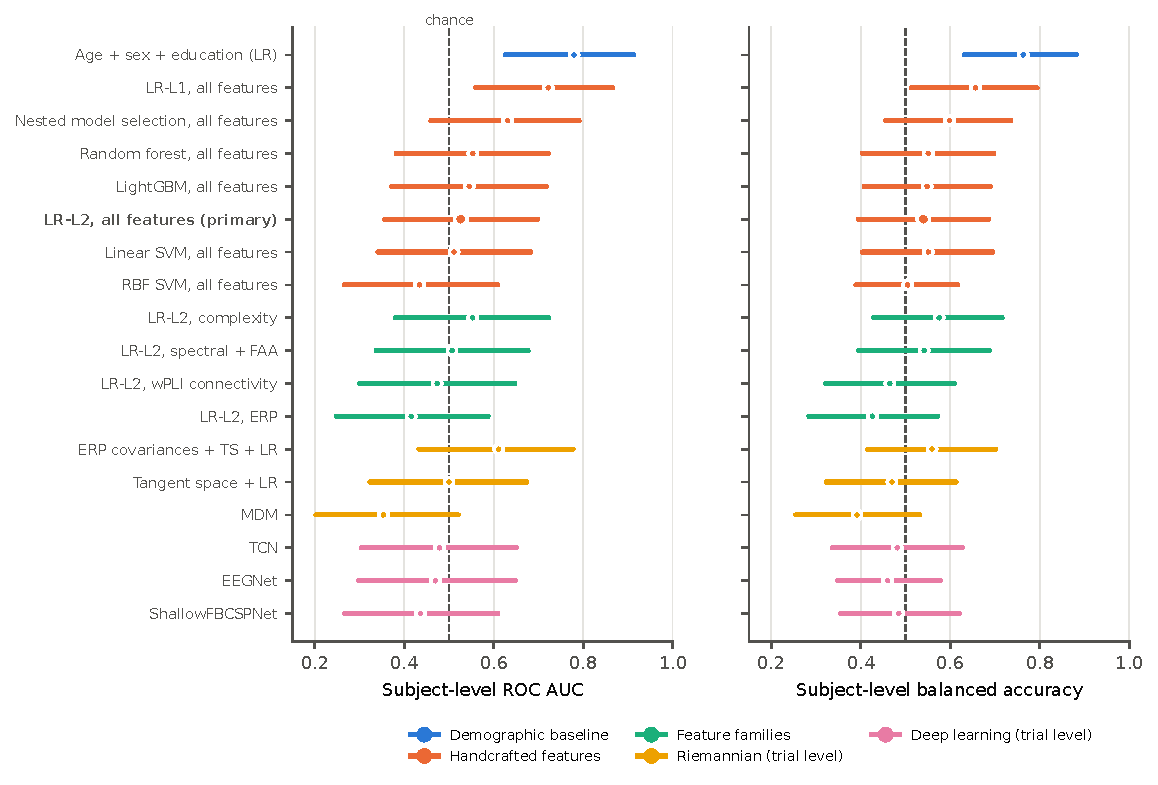
\includegraphics[width=\linewidth]{fig_model_comparison}
\caption{Participant-level ROC AUC (left) and balanced accuracy (right) with 95\% bootstrap CIs, for every model.
The dashed line marks chance. Only the demographic baseline (blue), which uses no EEG, has a CI clearly above
chance.}
\label{fig:models}
\end{figure}

\begin{table}[t]
\centering\scriptsize
\caption{Paired comparisons on identical participant folds. $\Delta$AUC is the mean per-fold difference
(model $-$ reference). $p_\text{corr}$ is from the corrected resampled $t$-test~\cite{nadeau2003inference}.
$p_\text{Holm}$ applies Holm's correction to the permutation $p$-values of the secondary models.}
\label{tab:cmp}
\begin{tabular}{@{}lrrrrrr@{}}
\toprule
 & \multicolumn{2}{c}{vs.\ primary} & \multicolumn{2}{c}{vs.\ demographics} & & \\
\cmidrule(lr){2-3}\cmidrule(lr){4-5}
Model & $\Delta$AUC & $p_\text{corr}$ & $\Delta$AUC & $p_\text{corr}$ & $p_\text{perm}$ & $p_\text{Holm}$ \\
\midrule
LR-L1, all features & +0.16 & 0.106 & -0.09 & 0.470 & 0.013 & 0.169 \\
Nested model selection, all features & +0.08 & 0.392 & -0.17 & 0.176 & 0.080 & 0.955 \\
Random forest, all features & +0.02 & 0.672 & -0.22 & 0.029 & 0.348 & 1.000 \\
LightGBM, all features & +0.01 & 0.944 & -0.24 & 0.020 & 0.353 & 1.000 \\
LR-L2, all features (primary) & -- & -- & -0.25 & 0.019 & 0.456 & -- \\
Linear SVM, all features & -0.13 & 0.422 & -0.38 & 0.004 & 0.479 & 1.000 \\
RBF SVM, all features & -0.13 & 0.429 & -0.38 & 0.008 & 0.572 & 1.000 \\
LR-L2, complexity & +0.06 & 0.517 & -0.19 & 0.107 & 0.705 & 1.000 \\
LR-L2, spectral + FAA & -0.01 & 0.903 & -0.26 & 0.011 & 0.325 & 1.000 \\
LR-L2, wPLI connectivity & -0.10 & 0.325 & -0.34 & 0.008 & 0.768 & 1.000 \\
LR-L2, ERP & -0.15 & 0.121 & -0.40 & 0.000 & 0.720 & 1.000 \\
ERP covariances + TS + LR & +0.08 & 0.455 & -0.17 & 0.164 & 0.159 & 1.000 \\
Tangent space + LR & -0.05 & 0.670 & -0.30 & 0.027 & 0.532 & 1.000 \\
MDM & -0.19 & 0.094 & -0.44 & 0.000 & 0.891 & 1.000 \\
TCN & -0.07 & 0.656 & -0.31 & 0.078 & -- & -- \\
EEGNet & -0.09 & 0.512 & -0.33 & 0.022 & -- & -- \\
ShallowFBCSPNet & -0.12 & 0.434 & -0.36 & 0.025 & -- & -- \\
\bottomrule
\end{tabular}
\end{table}

\begin{figure}[t]
\centering
\begin{subfigure}[t]{0.36\linewidth}
  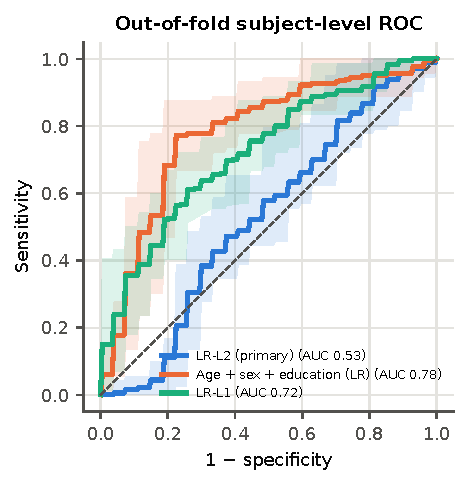
\includegraphics[width=\linewidth]{fig_roc}
  \caption{}
\end{subfigure}\hfill
\begin{subfigure}[t]{0.62\linewidth}
  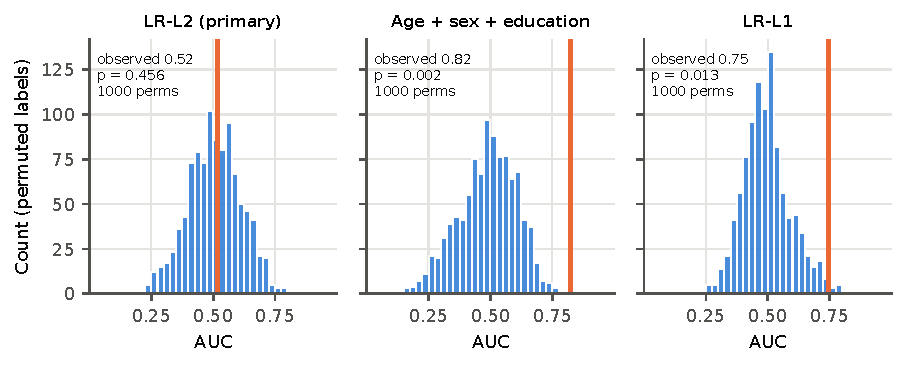
\includegraphics[width=\linewidth]{fig_permutation}
  \caption{}
\end{subfigure}
\caption{(a) Mean out-of-fold ROC curves across repetitions (band: 2.5--97.5\% range over repetitions).
(b) Permutation null distributions of the participant-level AUC, with the observed AUC (first repetition) marked.}
\label{fig:perm}
\end{figure}

\subsection{How much does trial-wise splitting inflate performance?}\label{sec:inflation}
Fig.~\ref{fig:inflation} contrasts the same two trial-level models under a trial-wise split, where trials of a
participant can fall in both training and test sets, and a subject-wise split.
\begin{itemize}
  \item \textbf{Tangent-space model.} Trial-level AUC was \InflTsLrTrialSplitTrialAuc{} with the trial-wise split and
        \InflTsLrSubjectSplitTrialAuc{} with the subject-wise split. Averaging trial probabilities per participant
        gave a participant-level AUC of \InflTsLrTrialSplitSubjectAuc{} under the trial-wise split, i.e.\ perfect
        apparent diagnosis, versus \InflTsLrSubjectSplitSubjectAuc{} under the subject-wise split.
  \item \textbf{Random forest on raw regional amplitudes}, the approach of many published studies and of an earlier
        unpublished analysis of these data by the author. Trial-level AUC was
        \InflRawamplitudeRfTrialSplitTrialAuc{} versus \InflRawamplitudeRfSubjectSplitTrialAuc, and participant-level
        AUC was \InflRawamplitudeRfTrialSplitSubjectAuc{} versus \InflRawamplitudeRfSubjectSplitSubjectAuc.
\end{itemize}
The trial-wise figures do not measure diagnosis. A classifier can recognise the \emph{participant} from the
individual statistics of their EEG, and the participant determines the label. Only the subject-wise figures answer
the clinical question.

The subject-wise participant-level AUC of the raw-amplitude random forest (\InflRawamplitudeRfSubjectSplitSubjectAuc)
is the highest of any EEG model. We do not interpret it as evidence of a diagnostic signal, for three reasons:
\begin{itemize}
  \item the model was included as a control, not pre-specified as a diagnostic model;
  \item it was evaluated with only three repetitions, and its post-hoc permutation test was borderline and did not
        survive multiplicity correction ($p=\AudRawRfP$, Holm $p=\AudRawRfPholm$; Section~\ref{sec:audit});
  \item it is one of many analyses, and for reference, 5\% of permutation runs of the primary pipeline exceeded AUC
        \PrimaryLrLAllNullQ.
\end{itemize}
It does suggest that the raw ERP waveform may be worth testing as a pre-specified hypothesis in independent data.

\begin{figure}[t]
\centering
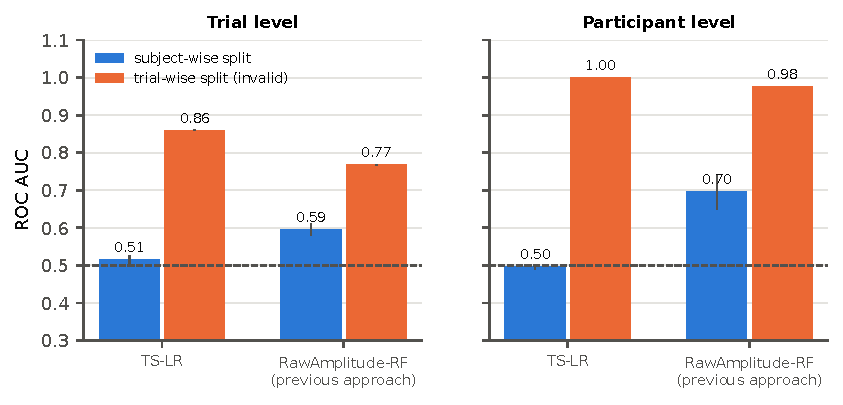
\includegraphics[width=0.85\linewidth]{fig_inflation}
\caption{AUC of the same models evaluated with a trial-wise split (invalid; trials of each participant appear in
training and test) and with a subject-wise split, at the trial level (left) and after averaging trial probabilities
per participant (right). Bars show means over three repetitions, with SD as error bars. The trial-wise split is shown
only to quantify the inflation.}
\label{fig:inflation}
\end{figure}

\subsection{Confounds and sensitivity analyses}
Table~\ref{tab:conf} reports whether the EEG features could predict variables other than diagnosis, using the
primary pipeline.
\begin{itemize}
  \item \textbf{Sex:} AUC $=\ConfSexAuc$ (\ConfSexAucLo--\ConfSexAucHi, $p=\ConfSexP$).
  \item \textbf{Age above the median:} \ConfAgeAuc{} ($p=\ConfAgeP$).
  \item \textbf{Recording period:} \ConfRecordingAuc{} ($p=\ConfRecordingP$).
\end{itemize}
EEG features thus carried information about sex, consistent with known sex differences in EEG amplitude and
spectra. Sex was balanced across groups (Table~\ref{tab:demo}), however, so it cannot explain a diagnostic signal,
and none was found. Neither age nor recording period was predictable from EEG.

Restricting the analysis to the \SensN{} participants recorded between June and August 2015 (\SensNMDD{} MDD), when
both groups were recorded in parallel, gave AUC $=\SensAuc$ (\SensAucLo--\SensAucHi, $p=\SensP$).

Including all 53 participants, with no exclusions, gave AUC $=\AllAuc$ (\AllAucLo--\AllAucHi, $p=\AllP$). The null
result is therefore not an artefact of the exclusion criteria. Primary-model AUC was similar in women
(\BySexFemaleAuc, $n=\BySexFemaleN$) and men (\BySexMaleAuc, $n=\BySexMaleN$).

\begin{table}[t]
\centering\small
\caption{Can the EEG features predict confounds? The primary pipeline (LR-L2, all features) was applied to
alternative targets, plus two sensitivity analyses of the MDD-vs-HC classification.}
\label{tab:conf}
\begin{tabular}{@{}lrll@{}}
\toprule
Target predicted from EEG features & $n_\text{pos}/n$ & AUC [95\% CI] & $p_\text{perm}$ \\
\midrule
sex (male) & 29/45 & 0.63 [0.45, 0.79] & 0.018 \\
age > median & 21/45 & 0.50 [0.33, 0.67] & 0.617 \\
recording period (>= Sep 2015) & 18/45 & 0.55 [0.37, 0.72] & 0.392 \\
\midrule
\multicolumn{4}{@{}l}{\textit{MDD vs.\ HC, primary pipeline, restricted subset}} \\
Recorded Jun--Aug 2015 & 9/25 & 0.46 [0.24, 0.70] & 0.517 \\
All 53 participants (no exclusions) & 24/53 & 0.57 [0.42, 0.72] & 0.278 \\
\bottomrule
\end{tabular}
\end{table}

\subsection{What, if anything, differs between groups?}
\paragraph{Model-based importance.} Permuting whole feature families in the test folds of the primary model
changed AUC by:
\begin{itemize}
  \item complexity: $\ImpComplexity$;
  \item spectral: $\ImpSpectral$;
  \item ERP: $\ImpErp$;
  \item connectivity: $\ImpConnectivity$.
\end{itemize}
All bootstrap intervals included zero (Fig.~\ref{fig:interp}a). SHAP values of the refitted primary model
(Fig.~\ref{fig:interp}b) were small in absolute terms, consistent with the strong regularisation selected.

\paragraph{Univariate effects.} \UniNSig{} of \UniNFeat{} features differed between groups at uncorrected $p<0.05$,
close to the $\approx14$ expected by chance. Only \UniNFdr{} survived false-discovery-rate correction: theta-band
wPLI between left central and left temporal regions ($d=\UniTopD$, $p_\text{FDR}=\UniTopPfdr$; Table~\ref{tab:uni}).

\paragraph{Spectral topography and ERPs.} Fig.~\ref{fig:topo} suggests higher beta and low-gamma power in MDD,
strongest at the edge of the montage, but no spatial cluster survived correction (minimum cluster
$p=\PowerClusterMinP$).

Group-average ERPs (Fig.~\ref{fig:erp}) showed the expected P1--N170 complex and a centro-parietal positivity in
both groups. Visually, MDD participants had a smaller late positivity at occipito-temporal sites, but the
spatio-temporal cluster test did not confirm any group difference (\ErpNClusters{} candidate clusters, minimum
$p=\ErpClusterMinP$).

\begin{figure}[t]
\centering
\begin{subfigure}[t]{0.40\linewidth}
  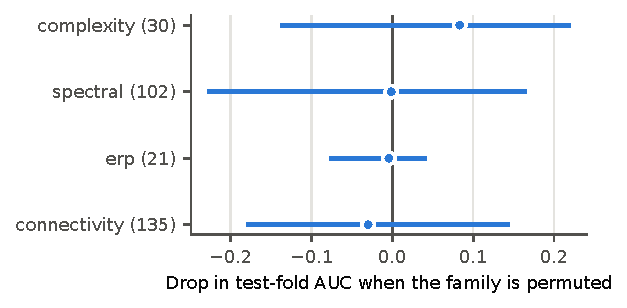
\includegraphics[width=\linewidth]{fig_family_importance}
  \caption{}
\end{subfigure}\hfill
\begin{subfigure}[t]{0.58\linewidth}
  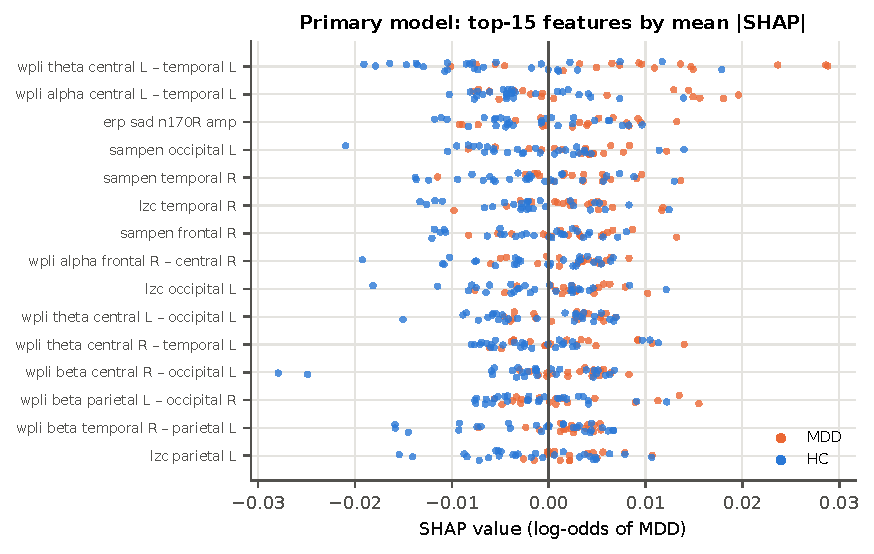
\includegraphics[width=\linewidth]{fig_shap}
  \caption{}
\end{subfigure}
\caption{(a) Drop in test-fold AUC of the primary model when each feature family is permuted jointly (mean and 95\%
interval over 50 outer folds; number of features in parentheses). (b) SHAP values of the primary model refitted on
all participants, for the 15 features with the largest mean $|$SHAP$|$ (descriptive).}
\label{fig:interp}
\end{figure}

\begin{figure}[t]
\centering
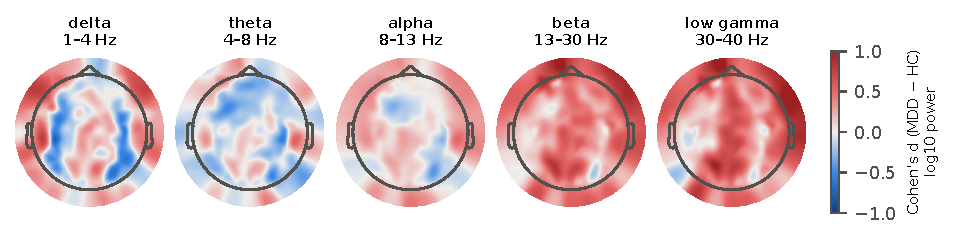
\includegraphics[width=\linewidth]{fig_topomaps_power}
\caption{Group differences in log band power per electrode (Cohen's $d$, MDD $-$ HC). Electrodes belonging to a
significant cluster (cluster permutation test, $p<0.05$) would be marked; none were.}
\label{fig:topo}
\end{figure}

\begin{figure}[t]
\centering
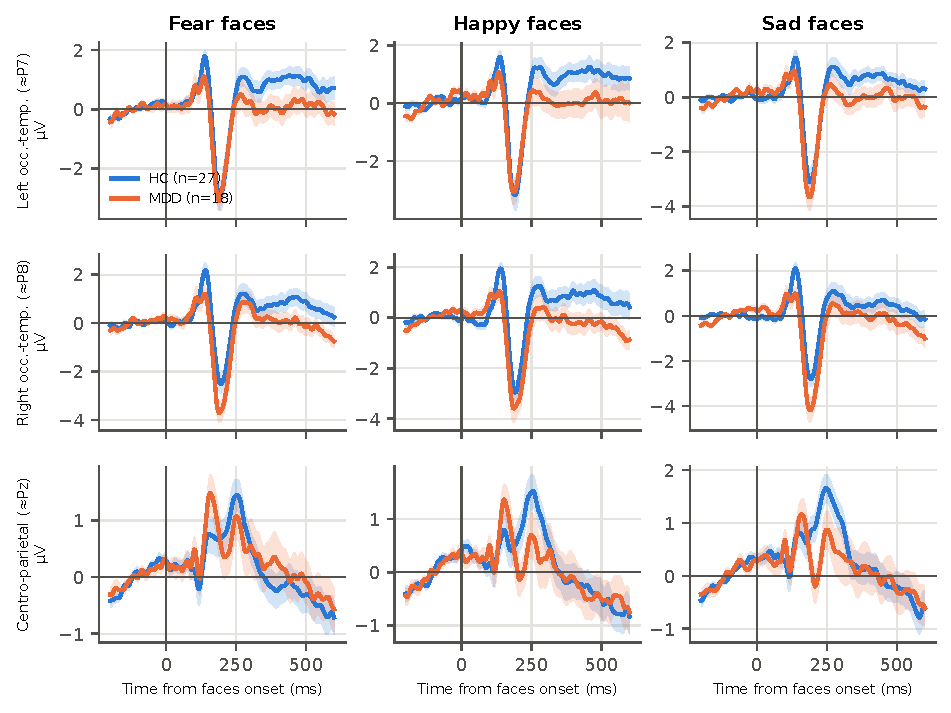
\includegraphics[width=\linewidth]{fig_erp_groups}
\caption{Grand-average ERPs ($\pm$SEM) per group and face condition, at the left and right occipito-temporal
clusters and the centro-parietal cluster. Shaded windows are the a-priori N170 (140--200~ms) and P300 (250--500~ms)
measurement windows.}
\label{fig:erp}
\end{figure}

\subsection{Post-hoc audit analyses (exploratory)}\label{sec:audit}
The analyses in this section were added after all pre-specified results were known (deviation D6;
Section~\ref{sec:audit-methods}). Table~\ref{tab:audit} lists the classification models. None of them changes the
conclusion.

\paragraph{Does EEG add to demographics?} No.
\begin{itemize}
  \item Adding all 288 EEG features to age, sex and education gave AUC $=\AudDemoPlusEEGAllAuc$
        (\AudDemoPlusEEGAllLo--\AudDemoPlusEEGAllHi). Permuting the EEG block gave $p=\AudDemoPlusEEGAllP$.
  \item Adding the compact set gave AUC $=\AudDemoPlusCompactAuc$ ($p=\AudDemoPlusCompactP$).
\end{itemize}
Both are \emph{below} the demographic baseline alone (\DemographicsLrAuc). With 45 participants, noisy EEG features
dilute rather than complement the demographic signal.

\paragraph{Is the null result an artefact of confounding or redundancy?} No.
\begin{itemize}
  \item EEG with age, sex and education regressed out inside each fold: AUC $=\AudEEGAlldeconfoundedAuc$
        ($p=\AudEEGAlldeconfoundedP$).
  \item PCA inside the fold: \AudEEGAllPCALRAuc{} ($p=\AudEEGAllPCALRP$).
  \item The compact theory-driven set, including the ERP contrasts between emotions, the aperiodic exponent, the
        alpha peak frequency and frontal-midline theta: \AudCompactLRAuc{} ($p=\AudCompactLRP$).
  \item Subject-level Riemannian model: \AudSubjectRiemannTSLRAuc{} ($p=\AudSubjectRiemannTSLRP$).
  \item Reaction times alone: \AudBehaviourRTLRAuc{} ($p=\AudBehaviourRTLRP$). Median RT was \AudRtMdd{} ms in MDD
        and \AudRtHc{} ms in HC ($p=\AudQRtIncP$).
\end{itemize}
The smallest uncorrected $p$ among these models was \AudMinP{}, and the smallest Holm-corrected $p$ was
\AudMinPholm.

\paragraph{Education as an EEG confound.} The EEG features did not predict education above the median: AUC
$=\AudEduAuc$ (\AudEduLo--\AudEduHi), $p=\AudEduP$. Only \AudEduNsig{} of 288 features correlated with education at
$p<0.05$, about the number expected by chance, and \AudEduNfdr{} survived FDR correction.

\paragraph{Residual muscle activity.} The EMG index, computed on the raw recordings, did not differ between groups
($p=\AudQEmgRelAllP$ in all 53 participants). It did, however, track the features that looked descriptively larger in
MDD (Fig.~\ref{fig:emg}):
\begin{itemize}
  \item mean sample entropy, $\rho=\AudEmgRSampen$;
  \item mean Lempel--Ziv complexity, $\rho=\AudEmgRLzc$;
  \item relative beta power, $\rho=\AudEmgRBeta$;
  \item relative 30--40~Hz power, $\rho=\AudEmgRGamma$;
  \item aperiodic exponent, $\rho=\AudEmgRApExp$ (all $p\le0.004$).
\end{itemize}
These families therefore index muscle tone as much as brain activity. The aperiodic exponent was nominally lower in
MDD ($p=\AudQApExpAllP$ in all 53; $p=\AudQApExpIncP$ in the 45 included). Given its correlation with the EMG index,
this cannot be attributed to cortical excitation--inhibition balance. The FDR-surviving wPLI feature was not related
to the EMG index ($\rho=\AudEmgRWpli$).

\paragraph{Signal quality before exclusion.} In all 53 participants, MDD and HC did not differ in:
\begin{itemize}
  \item retained trials ($p=\AudQTrialsAllP$);
  \item bad channels ($p=\AudQBadChAllP$);
  \item removed ICA components ($p=\AudQIcaAllP$) or ICLabel muscle components ($p=\AudQIcaMuscleAllP$).
\end{itemize}

\paragraph{Power.} The 95th percentile of the primary permutation null was AUC \AudPowThr. Even a perfect, already
trained score would exceed it with probability:
\begin{itemize}
  \item \AudPowIdealSeventy\% at true AUC 0.70;
  \item \AudPowIdealSeventyFive\% at 0.75;
  \item \AudPowIdealEighty\% at 0.80.
\end{itemize}
In the semi-synthetic analysis, where the primary pipeline has to learn the effect from 36 participants, power was
lower (Fig.~\ref{fig:power}a):
\begin{itemize}
  \item \AudSemiFivePower\% when the injected signal had an oracle AUC of \AudSemiFiveOracle;
  \item \AudSemiEightPower\% at oracle AUC \AudSemiEightOracle;
  \item \AudSemiTenPower\% at oracle AUC \AudSemiTenOracle.
\end{itemize}
The study could therefore only detect large effects. We extrapolated the same ideal score to larger samples, with
the same class ratio and one-sided $\alpha=0.05$. Reaching 80\% power would need about:
\begin{itemize}
  \item \AudNNeedSeventy{} participants for a true AUC of 0.70;
  \item \AudNNeedSixtyFive{} for 0.65;
  \item \AudNNeedSixty{} for 0.60.
\end{itemize}
These are optimistic lower bounds, because a pipeline that also has to learn the effect needs more.

\paragraph{Learning curve.} Between 12 and 36 training participants (Fig.~\ref{fig:power}b):
\begin{itemize}
  \item the primary model moved from AUC \AudLcPrimMin{} to \AudLcPrimMax;
  \item the demographic model moved from \AudLcDemoMin{} to \AudLcDemoMax.
\end{itemize}

\paragraph{Why trial-wise splits inflate.} A classifier on single-trial regional covariances identified \emph{which}
of the 45 participants produced a trial with \AudIdentAcc\% accuracy (chance \AudIdentChance\%). Individual EEG
signatures are thus highly distinctive, which explains the perfect participant-level AUC under trial-wise splitting
(Section~\ref{sec:inflation}).

\paragraph{Raw-amplitude random forest.} With the settings of its first repetition (AUC \AudRawRfObs), a permutation
test of the full subject-wise pipeline gave $p=\AudRawRfP$. The test used \AudRawRfN{} permutations, of which
\AudRawRfExceed{} reached the observed AUC, and the null 95th percentile was \AudRawRfQ. This is the only nominally
significant EEG result of the audit, but it is fragile:
\begin{itemize}
  \item with so few permutations, the 95\% interval for the exceedance probability extends to \AudRawRfPciHi;
  \item after Holm correction across the \AudRawRfFamily{} exploratory models it is $p=\AudRawRfPholm$;
  \item the model was not pre-specified, and a 288-feature linear model on summaries of the same data was at chance.
\end{itemize}
We therefore treat the raw ERP waveform as the most promising hypothesis this study generates, to be tested in
independent data, and not as a finding.

\begin{table}[t]
\centering\scriptsize
\setlength{\tabcolsep}{3pt}
\caption{Exploratory post-hoc models (D6), on the same folds as Table~\ref{tab:main}. $p_\text{perm}$: 1{,}000
permutations of the full nested pipeline. For the two incremental models the EEG block is permuted instead of the
labels. $p_\text{Holm}$ is computed across these seven models. $\Delta$AUC is the difference from the demographic
baseline, with the corrected resampled $t$-test.}
\label{tab:audit}
\begin{tabular}{@{}lccccc@{}}
\toprule
Model (exploratory, post hoc) & AUC [95\% CI] & BalAcc & $p_\text{perm}$ & $p_\text{Holm}$ & $\Delta$AUC vs demo ($p_\text{corr}$) \\
\midrule
Demographics + all 288 EEG features & 0.52 [0.35, 0.69] & 0.54 & 0.746 & 1.000 & -0.25 (0.014) \\
Demographics + compact EEG set & 0.59 [0.42, 0.75] & 0.59 & 0.584 & 1.000 & -0.17 (0.089) \\
EEG 288, age/sex/education regressed out in-fold & 0.49 [0.32, 0.66] & 0.50 & 0.703 & 1.000 & -0.28 (0.009) \\
EEG 288, PCA (in-fold) + LR & 0.58 [0.42, 0.75] & 0.58 & 0.381 & 1.000 & -0.18 (0.085) \\
Compact theory-driven EEG set (36) & 0.51 [0.34, 0.68] & 0.53 & 0.502 & 1.000 & -0.27 (0.009) \\
Reaction times only (8) & 0.44 [0.27, 0.62] & 0.49 & 0.726 & 1.000 & -0.37 (0.002) \\
Subject-mean covariance, tangent space + LR & 0.53 [0.35, 0.70] & 0.49 & 0.064 & 0.448 & -0.28 (0.065) \\
\bottomrule
\end{tabular}
\end{table}

\begin{figure}[t]
\centering
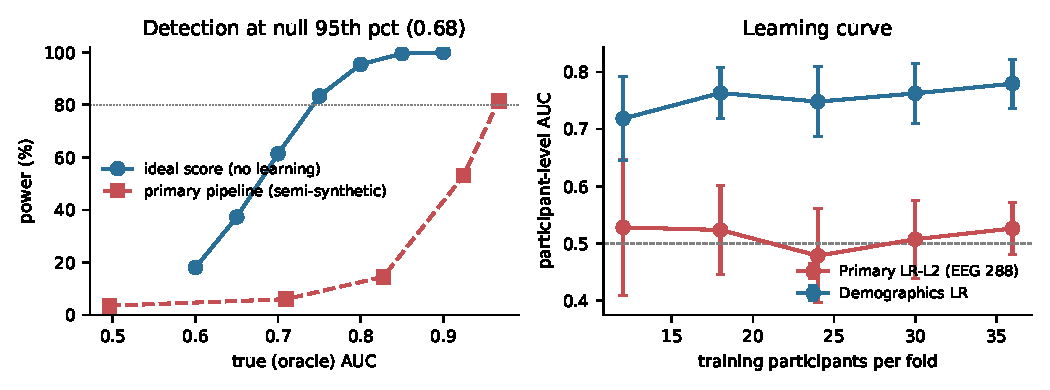
\includegraphics[width=\linewidth]{fig_power_curve}
\caption{(a) Probability of exceeding the 95th percentile of the permutation null, as a function of the true AUC. Blue:
an ideal pre-trained score. Red: the primary pipeline learning an injected effect, semi-synthetic. (b) Learning curve
(mean $\pm$ SD over 10 repetitions).}
\label{fig:power}
\end{figure}

\begin{figure}[t]
\centering
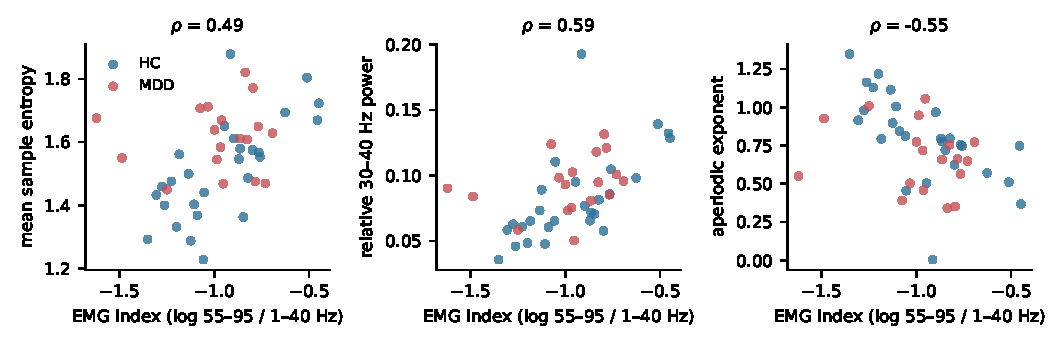
\includegraphics[width=\linewidth]{fig_emg}
\caption{EMG index (raw recordings) against global sample entropy, relative 30--40~Hz power and the aperiodic
exponent in the 45 included participants. $\rho$: Spearman correlation.}
\label{fig:emg}
\end{figure}

\section{Discussion}

\subsection{Main finding}
Under a strictly participant-wise, pre-specified protocol, task EEG from the MODMA dot-probe recordings did not
separate MDD from healthy controls better than chance. The conclusion holds across all model types tested:
\begin{itemize}
  \item the pre-specified primary model and every feature family on its own;
  \item linear, kernel and tree-based classifiers;
  \item Riemannian models and three deep networks trained on the full 128-channel epochs.
\end{itemize}
The one nominally significant secondary result (L1-regularised logistic regression) did not survive correction for
the number of secondary models. The honest estimate of picking the best model, obtained by nested model selection,
fell to \NestedmodelselectionAllAuc, with a confidence interval including chance.

By contrast, three demographic variables (age, sex and education) reached AUC \DemographicsLrAuc. Any EEG model that
claims diagnostic value on this dataset should be benchmarked against this figure, not only against 0.5.

These findings agree with reviews describing EEG markers of depression as small and heterogeneous
effects~\cite{olbrich2013eeg,deaguiar2019review,simmatis2023technical}. They also agree with the meta-analytic null
result for frontal alpha asymmetry~\cite{vandervinne2017faa}. They do not agree with the near-perfect accuracies often
reported for EEG-based depression detection~\cite{ay2019automated}.

\subsection{Why do published accuracies differ so much?}
Our inflation control offers a direct explanation. On the same data, the tangent-space model evaluated with a
trial-wise split ranked every participant correctly (participant-level AUC \InflTsLrTrialSplitSubjectAuc;
trial-level \InflTsLrTrialSplitTrialAuc). Evaluated on held-out participants, it was at chance
(\InflTsLrSubjectSplitSubjectAuc).

When epochs of one person appear in both training and test sets, the classifier only needs to recognise the person,
and every person carries one label. Individual EEG signatures are highly distinctive, so this task is easy, and it says
nothing about diagnosing a new patient~\cite{saeb2017need,brookshire2024leakage}. Reported accuracies therefore cannot
be interpreted unless the split is stated to be across participants. In this light, values above 95\% on datasets of
a few dozen participants should be regarded with suspicion.

\subsection{Model selection and multiplicity}
With $n=\NIncluded$, sampling noise alone produces large AUCs: under label permutation, the primary pipeline exceeded
AUC \PrimaryLrLAllNullQ{} in 5\% of runs. Across 18 configurations, some will exceed that by chance. Reporting the best of them, here L1-LR at AUC \LrLAllAuc, would have yielded a publishable but
misleading result.

Three elements of the design guard against this:
\begin{itemize}
  \item a primary model and outcome fixed before any result existed;
  \item multiplicity correction across secondary models;
  \item a nested estimate of the selection procedure itself~\cite{cawley2010overfitting}.
\end{itemize}
We recommend all three as standard practice for small clinical EEG datasets.

\subsection{Confounds}
The groups differed in education and, partly, in recording period: some months contain only patients or only
controls. In principle, period effects (equipment state, staff, season) could produce group differences unrelated to
depression.

Two observations make this unlikely to be the explanation here. First, the EEG features did not predict recording
period above chance. Second, the analysis restricted to the months in which both groups were recorded was no more
successful than the full analysis.

The signal-quality measures did not differ between groups. Even so, one descriptive pattern deserves caution:
\begin{itemize}
  \item MDD participants showed numerically higher beta and low-gamma power, strongest at peripheral electrodes;
  \item they also showed higher entropy and Lempel--Ziv complexity, the family whose permutation importance was
        largest, though not significant.
\end{itemize}
Both patterns are also typical signatures of residual muscle activity. ICA with ICLabel removes the clearest muscle
components but not all EMG. Any future report of high-frequency or complexity differences in these data should
therefore rule out muscle tension before attributing them to depression.

The single connectivity feature that survived FDR correction (left central--temporal theta wPLI) was not robustly
used by any model. It should be considered a hypothesis for replication, not a finding.

\subsection{Limitations}
\begin{itemize}
  \item \textbf{Sample size.} With \NIncludedMDD{} MDD and \NIncludedHC{} HC participants after exclusion, the
        participant-level confidence intervals are wide: for the primary model,
        \PrimaryLrLAllAucLo--\PrimaryLrLAllAucHi. A modest true effect, around AUC 0.6, cannot be excluded. Our
        conclusion is that these data provide no evidence of a diagnostic signal, not that none exists.
  \item \textbf{Single site and single task.} All data come from one site, one EEG system and one paradigm. Clinical
        details that may modulate EEG are not modelled, notably medication status and illness duration.
  \item \textbf{Asymmetric exclusions.} The pre-specified quality criteria excluded more patients than controls. The
        analysis on all 53 participants, however, gave the same conclusion.
  \item \textbf{Deep learning budget.} For computational reasons, the deep networks were evaluated with 3 rather than
        10 repetitions and without permutation tests. Their confidence intervals all included chance, and their point
        estimates were below that of the primary model.
  \item \textbf{Feature space.} The features were fixed a priori from the literature. Other representations could
        perform better, but searching for them on the same 45 participants would reintroduce the selection bias this
        study was designed to avoid.
\end{itemize}

\subsection{Conclusion}
Evaluated rigorously on participants never seen by the model, 128-channel task EEG from the MODMA dot-probe dataset
did not distinguish major depression from healthy controls, and was outperformed by a demographic baseline. The large
gap between trial-wise and participant-wise estimates on the same data shows how evaluation choices can manufacture
apparent diagnostic accuracy. Credible progress towards EEG markers of depression will require participant-wise
evaluation, pre-specified analyses, demographic baselines and substantially larger, multi-site samples.


\section*{Code and data availability}
All code, the analysis plan (fixed and version-controlled before any result was produced) and the list of deviations
are available at \url{https://github.com/nicolasrodriguezco/eeg-mdd-pipeline}, with a companion book documenting code, methods and results at \url{https://nicolasrodriguezco.github.io/eeg-mdd-pipeline}. The EEG data belong to the MODMA project~\cite{cai2022modma} and were
obtained from its maintainers for academic use; they are not redistributed.

\section*{Acknowledgements}
This work grew out of a research-seminar project at Universidad del Norte. The author thanks Dr.\ Karen Fl\'orez for
her supervision of that project, and the MODMA team for making the data available for academic research.

\section*{Use of AI tools}
An AI coding assistant was used to write and test the analysis code and to draft the text. All analysis
decisions, code and results were checked by the author, and every number in this paper is generated
programmatically from saved outputs.

\section*{Disclaimer}
This work is a methodological study. The models described here are \emph{not} diagnostic tools and must not be
used for clinical decision-making.

\bibliographystyle{unsrtnat}
\bibliography{refs}

\appendix
\section{Deviations from the pre-specified plan}\label{app:deviations}
Deviations D1--D4 were decided before any model had been trained; at that point only the preprocessing log had been
inspected. D5 was decided after the subject-level models had been evaluated but before any result of the affected
(Riemannian) models existed.

\begin{enumerate}
  \item[D1] \textbf{Bad-channel detector.}
        \begin{itemize}
          \item \emph{Problem:} the pre-specified rule (flat signal, robust log-SD $z>5$, median neighbour correlation
                $<0.4$) flagged up to 48 of 129 channels in a recording. Of all flags, 94\% came from the
                neighbour-correlation criterion, and they included channels adjacent to the vertex reference with
                \emph{negative} neighbour correlations. Whole-recording correlation is not a valid quality measure on
                reference-dominated, artefact-laden data.
          \item \emph{Change:} the rule was replaced by the PREP implementation~\cite{bigdely2015prep}.
          \item \emph{Unchanged:} the 20\% exclusion threshold.
        \end{itemize}
  \item[D2] \textbf{Re-run.} Fourteen participants were re-run after an infrastructure failure: a library was being
        installed during the first run. Since D1 required a full re-run anyway, all 53 were re-processed.
  \item[D3] \textbf{Added model.} The ERP-covariance Riemannian model was added as a secondary model.
  \item[D4] \textbf{Added sensitivity analysis.} Exclusions affected \NExcludedMDD{} MDD and \NExcludedHC{} HC
        participants, so we added a sensitivity analysis of the primary model on all 53 participants.
  \item[D5] \textbf{Computational budget of the Riemannian models.}
        \begin{itemize}
          \item \emph{Problem:} timing one outer fold showed that the full protocol (10 repetitions plus 200
                permutations, i.e.\ 1{,}050 outer folds per model) would take more than 12~h, mostly because
                per-trial covariances were recomputed in every inner-loop fit.
          \item \emph{Change 1 (no effect on results):} for the tangent-space and MDM models, per-trial OAS
                covariances were computed once. Each covariance depends only on its own trial, so this involves no
                learning across samples; the tangent-space reference point, scaling, classifier and MDM centroids
                were still fitted inside each training fold. A unit test verifies identical predictions.
          \item \emph{Change 2:} the ERP-covariance model, whose class prototypes depend on labels and must be
                recomputed within each fold, used a fixed regularisation $C=0.1$ instead of an inner grid. A value
                fixed in advance cannot inflate performance; at worst it is slightly sub-optimal.
        \end{itemize}
  \item[D6] 	extbf{Post-hoc audit analyses (exploratory).} After all pre-specified results were known, an internal
        audit added the analyses of Sections~
ef{sec:audit-methods} and~
ef{sec:audit}. They do not replace,
        re-rank or re-threshold any pre-specified result. They are Holm-corrected among themselves and labelled
        exploratory throughout.
\end{enumerate}

\section{Preprocessing quality}
\begin{figure}[h]
\centering
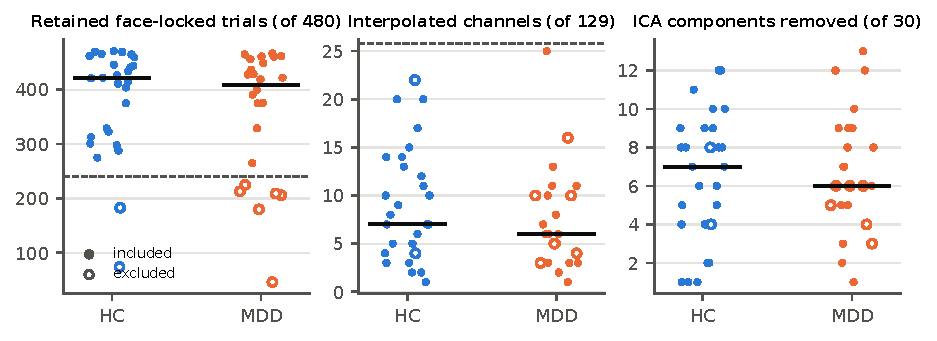
\includegraphics[width=\linewidth]{fig_quality}
\caption{Signal quality per participant: retained face-locked trials, interpolated channels and removed ICA
components. Open markers show participants excluded by the pre-specified criteria (dashed lines). Horizontal bars
are group medians.}
\label{fig:quality}
\end{figure}

\begin{figure}[h]
\centering
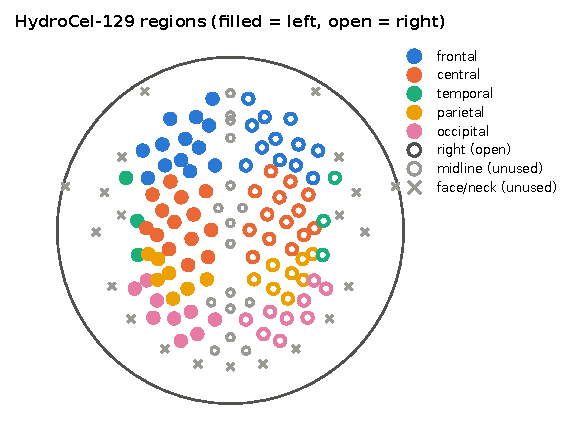
\includegraphics[width=0.55\linewidth]{fig_regions}
\caption{Assignment of HydroCel-129 electrodes to the ten regions, obtained by nearest 10--10 anchor on the fitted
head sphere. Filled markers are left-hemisphere electrodes and open markers right-hemisphere electrodes. Grey
electrodes (midline, and the face/neck ring more than \SI{115}{\degree} from the vertex) are not used for regional
features.}
\label{fig:regions}
\end{figure}

\section{Univariate group differences}
\begin{table}[h]
\centering\small
\caption{The ten features with the smallest uncorrected Mann--Whitney $p$ (MDD vs.\ HC, included participants).
$p_\text{FDR}$ is Benjamini--Hochberg corrected over all 288 features.}
\label{tab:uni}
\begin{tabular}{@{}llrrr@{}}
\toprule
Feature & Family & Cohen's $d$ & $p$ & $p_\text{FDR}$ \\
\midrule
\texttt{wpli\_theta\_central\_L\_\_temporal\_L} & connectivity & 1.38 & $<$0.001 & 0.04 \\
\texttt{sampen\_occipital\_L} & complexity & 0.79 & 0.003 & 0.45 \\
\texttt{rel\_lowgamma\_occipital\_L} & spectral & 0.57 & 0.005 & 0.47 \\
\texttt{sampen\_temporal\_R} & complexity & 0.76 & 0.009 & 0.62 \\
\texttt{rel\_beta\_occipital\_L} & spectral & 0.69 & 0.012 & 0.66 \\
\texttt{wpli\_beta\_central\_R\_\_occipital\_L} & connectivity & -0.70 & 0.018 & 0.66 \\
\texttt{sampen\_parietal\_L} & complexity & 0.72 & 0.020 & 0.66 \\
\texttt{lzc\_occipital\_L} & complexity & 0.71 & 0.022 & 0.66 \\
\texttt{lzc\_temporal\_R} & complexity & 0.72 & 0.022 & 0.66 \\
\texttt{pow\_lowgamma\_occipital\_L} & spectral & 0.64 & 0.024 & 0.66 \\
\bottomrule
\end{tabular}
\end{table}

\section{Feature dictionary}\label{app:dictionary}
Every subject-level feature is computed per participant without labels. Names join the family, the band or measure and the region with underscores, for example
\texttt{pow\_alpha\_frontal\_L}. Regions are frontal, central, temporal, parietal and occipital, each
left (L) or right (R).

\begin{table}[h]
\centering\scriptsize
\caption{The 288 pre-specified subject-level features.}
\label{tab:dictionary}
\begin{tabular}{@{}p{3.3cm}rp{9.2cm}@{}}
\toprule
Name pattern & $n$ & Definition and interpretation \\
\midrule
\texttt{pow\_<band>\_<region>} & 50 & $\log_{10}$ absolute Welch power (\si{\micro\volt\squared}) in delta 1--4, theta
  4--8, alpha 8--13, beta 13--30 and low gamma 30--40~Hz, averaged over the region's electrodes. Depends on skull
  thickness and impedance as well as on brain activity. \\
\texttt{rel\_<band>\_<region>} & 50 & Band power divided by 1--40~Hz power. Removes individual scale. The five
  bands of a region sum to $\approx0.94$, so they are nearly collinear. \\
\texttt{faa\_F3F4}, \texttt{faa\_F7F8} & 2 & Frontal alpha asymmetry, $\ln\alpha_R-\ln\alpha_L$ (E124/E24,
  E122/E33). Lower values mean relatively less left-frontal activity, which approach--withdrawal theory predicts in
  depression. \\
\texttt{erp\_<cond>\_n170L/R\_amp}, \texttt{\_lat} & 12 & Minimum amplitude and its latency at 140--200~ms, at
  clusters around P7/P8, per condition (fear, happy, sad). Structural face encoding. \\
\texttt{erp\_<cond>\_p300\_amp}, \texttt{\_lat} & 6 & Mean amplitude (250--500~ms) and peak latency at a
  centro-parietal cluster around Pz. Attentional allocation. \\
\texttt{erp\_<cond>\_lpp\_amp} & 3 & Mean amplitude at 400--600~ms, same cluster. Sustained motivated attention.
  Overlaps the P300 window ($r\approx0.9$ with P300 amplitude). \\
\texttt{wpli\_<band>\_<A>\_\_<B>} & 135 & Weighted phase-lag index between region-mean signals (45 pairs, theta,
  alpha and beta), multitaper over 2-s segments. It ignores zero-lag coupling, which reduces volume conduction. \\
\texttt{sampen\_<region>} & 10 & Sample entropy ($m=2$, $r=0.2$\,SD). Signal unpredictability. \\
\texttt{hfd\_<region>} & 10 & Higuchi fractal dimension ($k_\text{max}=10$). Signal roughness. \\
\texttt{lzc\_<region>} & 10 & Normalised Lempel--Ziv complexity of the median-binarised signal. \\
\bottomrule
\end{tabular}
\end{table}

Spectral, connectivity and complexity features are computed on the cleaned \emph{task} recording, not at rest.
Complexity and high-frequency power are sensitive to residual muscle activity (Section~\ref{sec:audit}).


\end{document}
